\chapter{Perancangan}
\label{chap:perancangan}

\section{Perancangan Kelas Akibat Kurikulum 2018}

Pada subbab ini akan menjelaskan perancangan kelas akibat kurikulum 2018 dari hasil analisis pada subbab \ref{subbab:analisissiamodels} \& \ref{subbab:analisisifstudentportal}. Diagram kelas akibat kurikulum 2018 dibagi menjadi beberapa bagian yang dapat dilihat pada gambar \ref{fig:siamodels_class_2018} untuk diagram kelas SIAModels yang berubah pada kelas \texttt{Nilai} dan untuk diagram kelas lengkapnya dapat dilihat pada gambar \ref{fig:2_siamodels_class}. Gambar \ref{fig:siamodels_class_2018_kurikulum_1}, \ref{fig:siamodels_class_2018_kurikulum_2}, \ref{fig:siamodels_class_2018_kurikulum_3}, \ref{fig:siamodels_class_2018_kurikulum_4}, dan \ref{fig:siamodels_class_2018_kurikulum_5} untuk diagram kelas yang merepresentasikan mata kuliah pada kurikulum 2018. Deskripsi kelas berserta fungsi dari diagram kelas tersebut adalah sebagai berikut:

\begin{figure}[H]
\centering
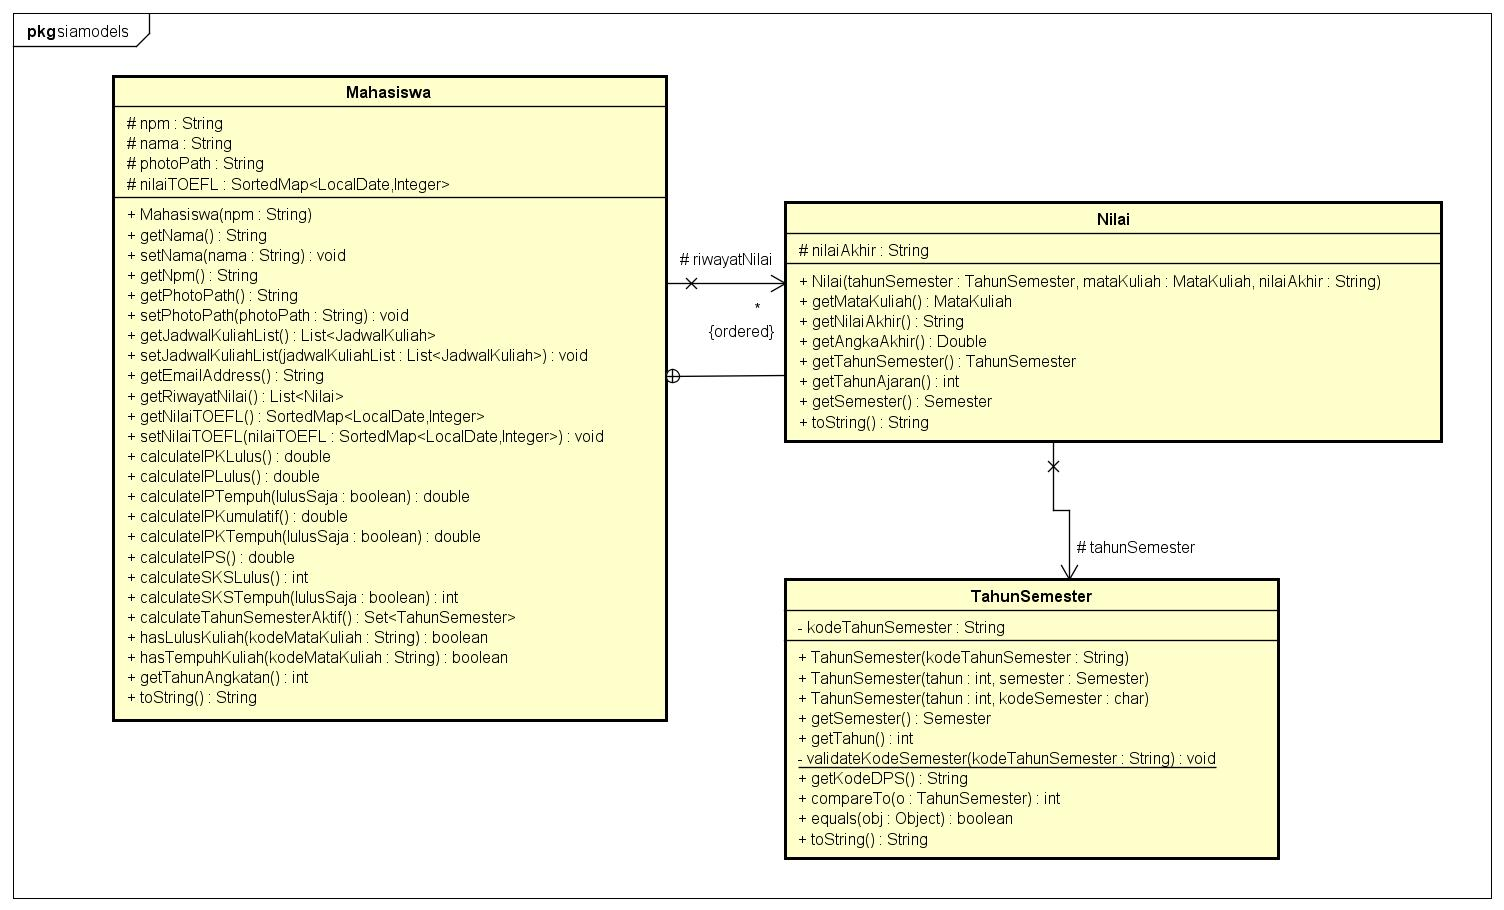
\includegraphics[scale=0.3]{Gambar/class-diagram-siamodels-new}
\caption{Diagram Kelas SIAModels Bagian \texttt{Nilai}}
\label{fig:siamodels_class_2018}
\end{figure}

\begin{figure}[H]
\centering
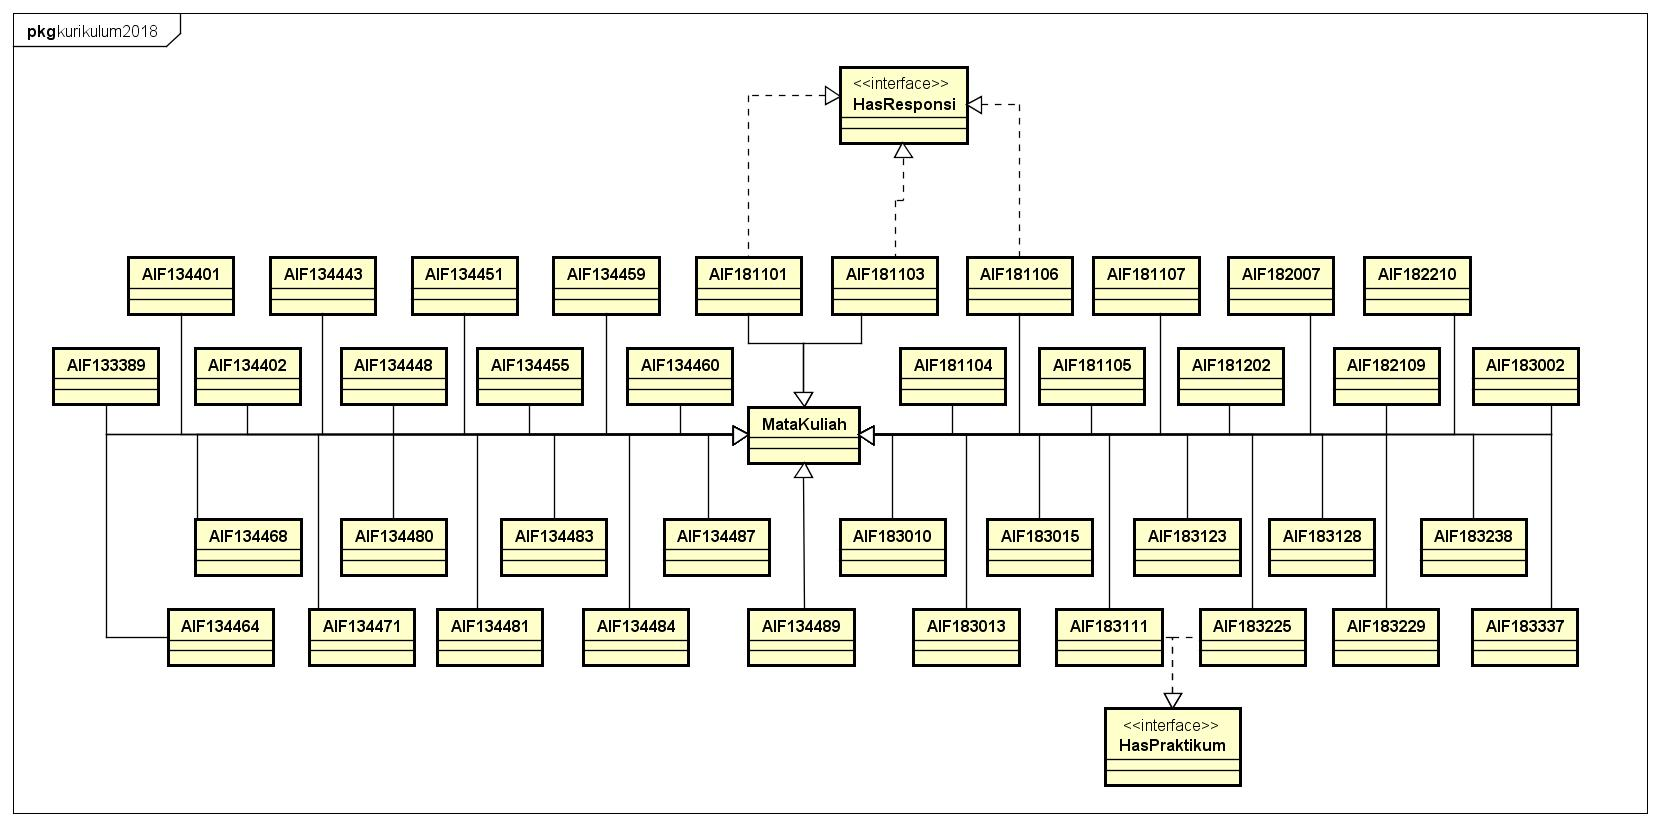
\includegraphics[scale=0.28]{Gambar/class-diagram-siamodels-mk-kurikulum-2018-2}
\caption{Diagram Kelas SIAModels \textit{Package} \texttt{kurikulum2018} (1/5)}
\label{fig:siamodels_class_2018_kurikulum_1}
\end{figure}

\begin{figure}[H]
\centering
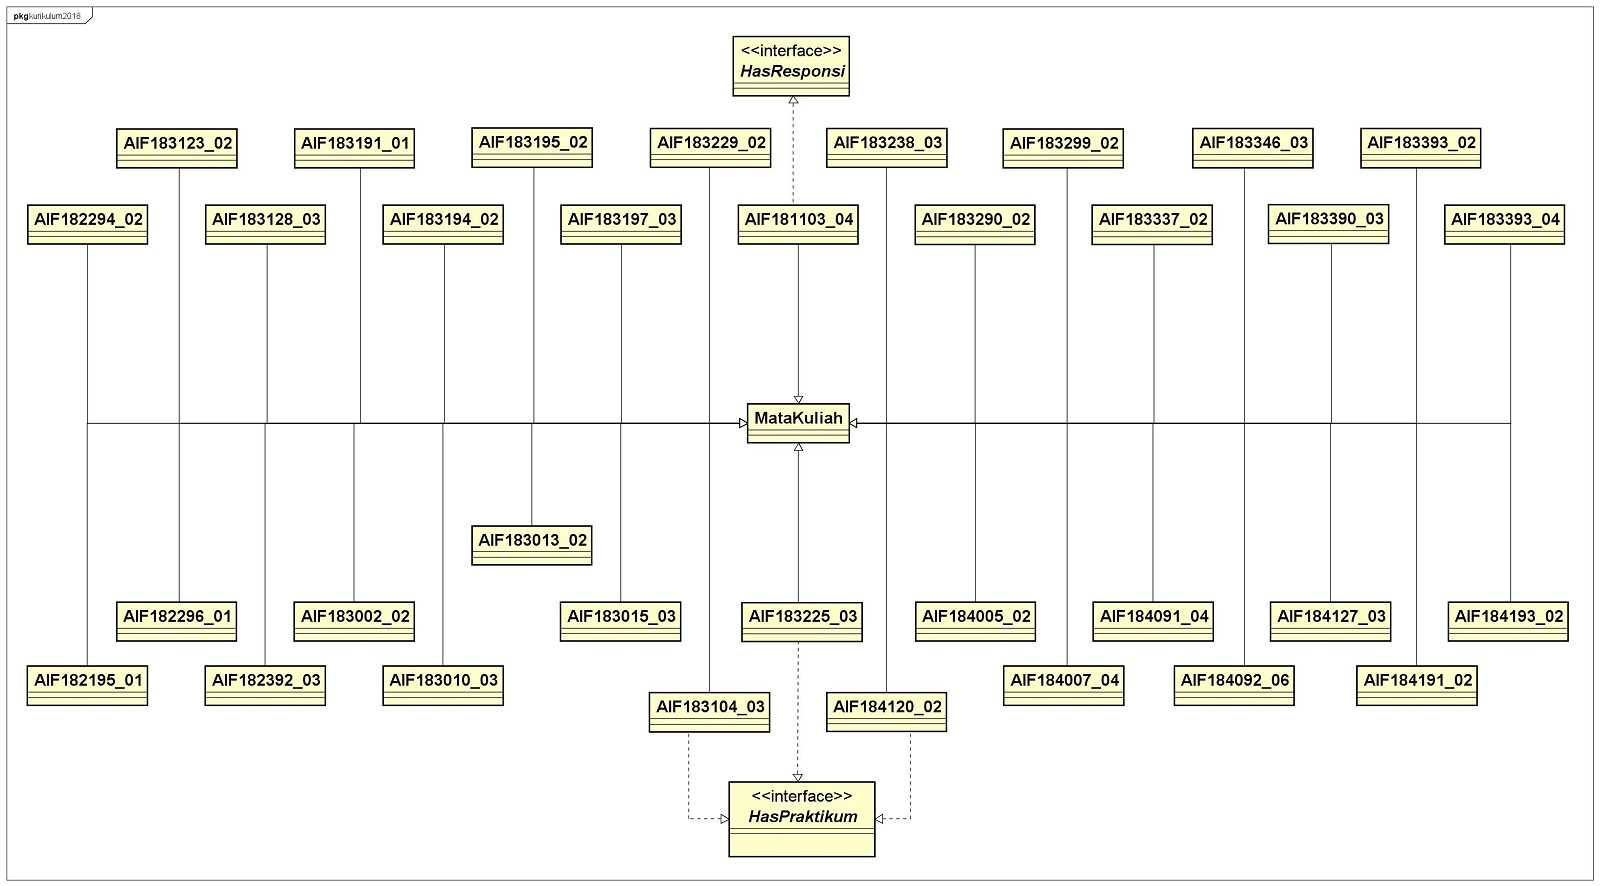
\includegraphics[scale=0.29]{Gambar/class-diagram-siamodels-mk-kurikulum-2018-1}
\caption{Diagram Kelas SIAModels \textit{Package} \texttt{kurikulum2018} (2/5)}
\label{fig:siamodels_class_2018_kurikulum_2}
\end{figure}

\begin{figure}[H]
\centering
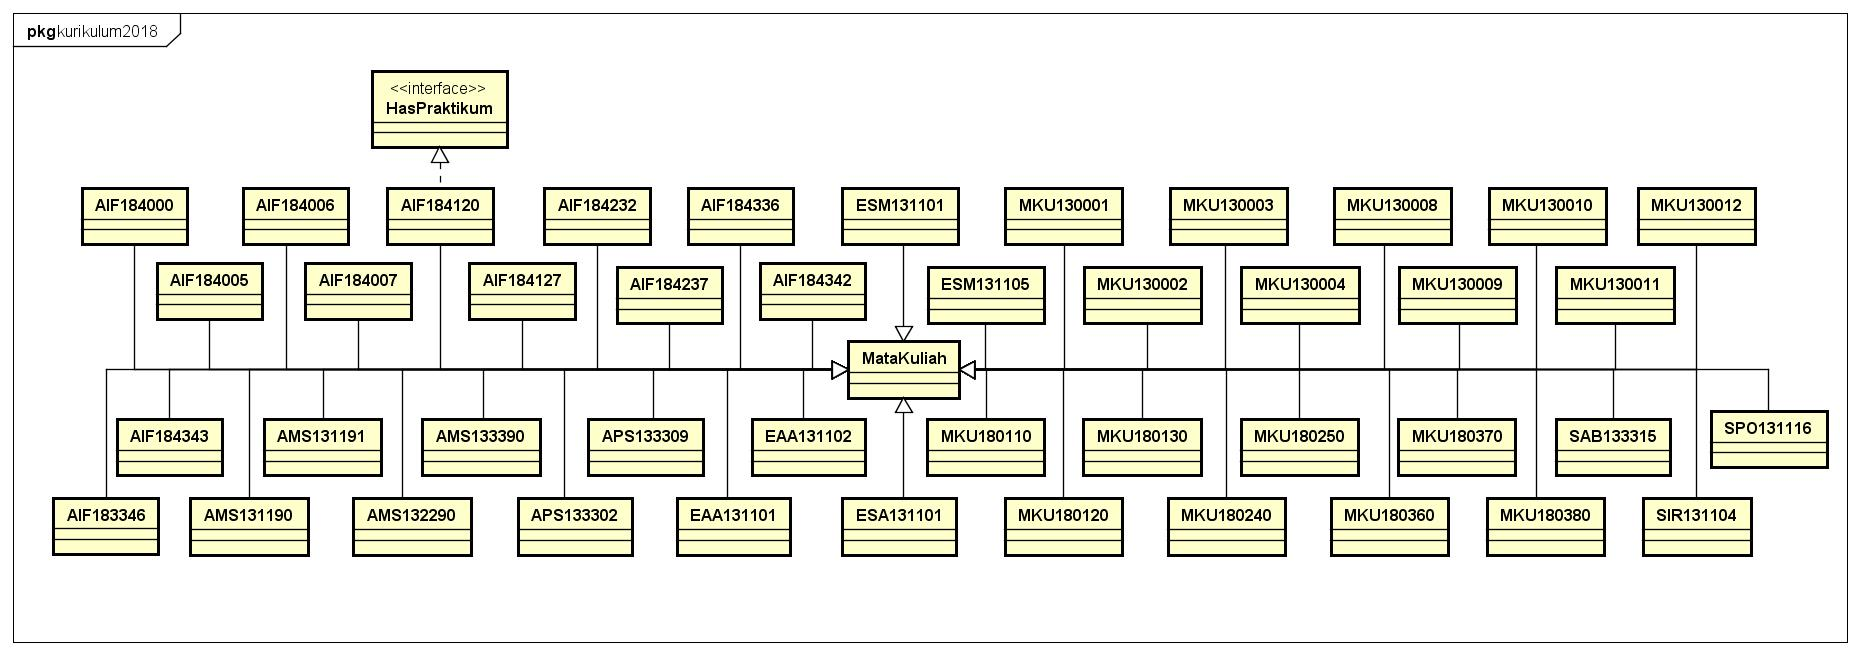
\includegraphics[scale=0.25]{Gambar/class-diagram-siamodels-mk-kurikulum-2018-3}
\caption{Diagram Kelas SIAModels \textit{Package} \texttt{kurikulum2018} (3/5)}
\label{fig:siamodels_class_2018_kurikulum_3}
\end{figure}

\begin{figure}[H]
\centering
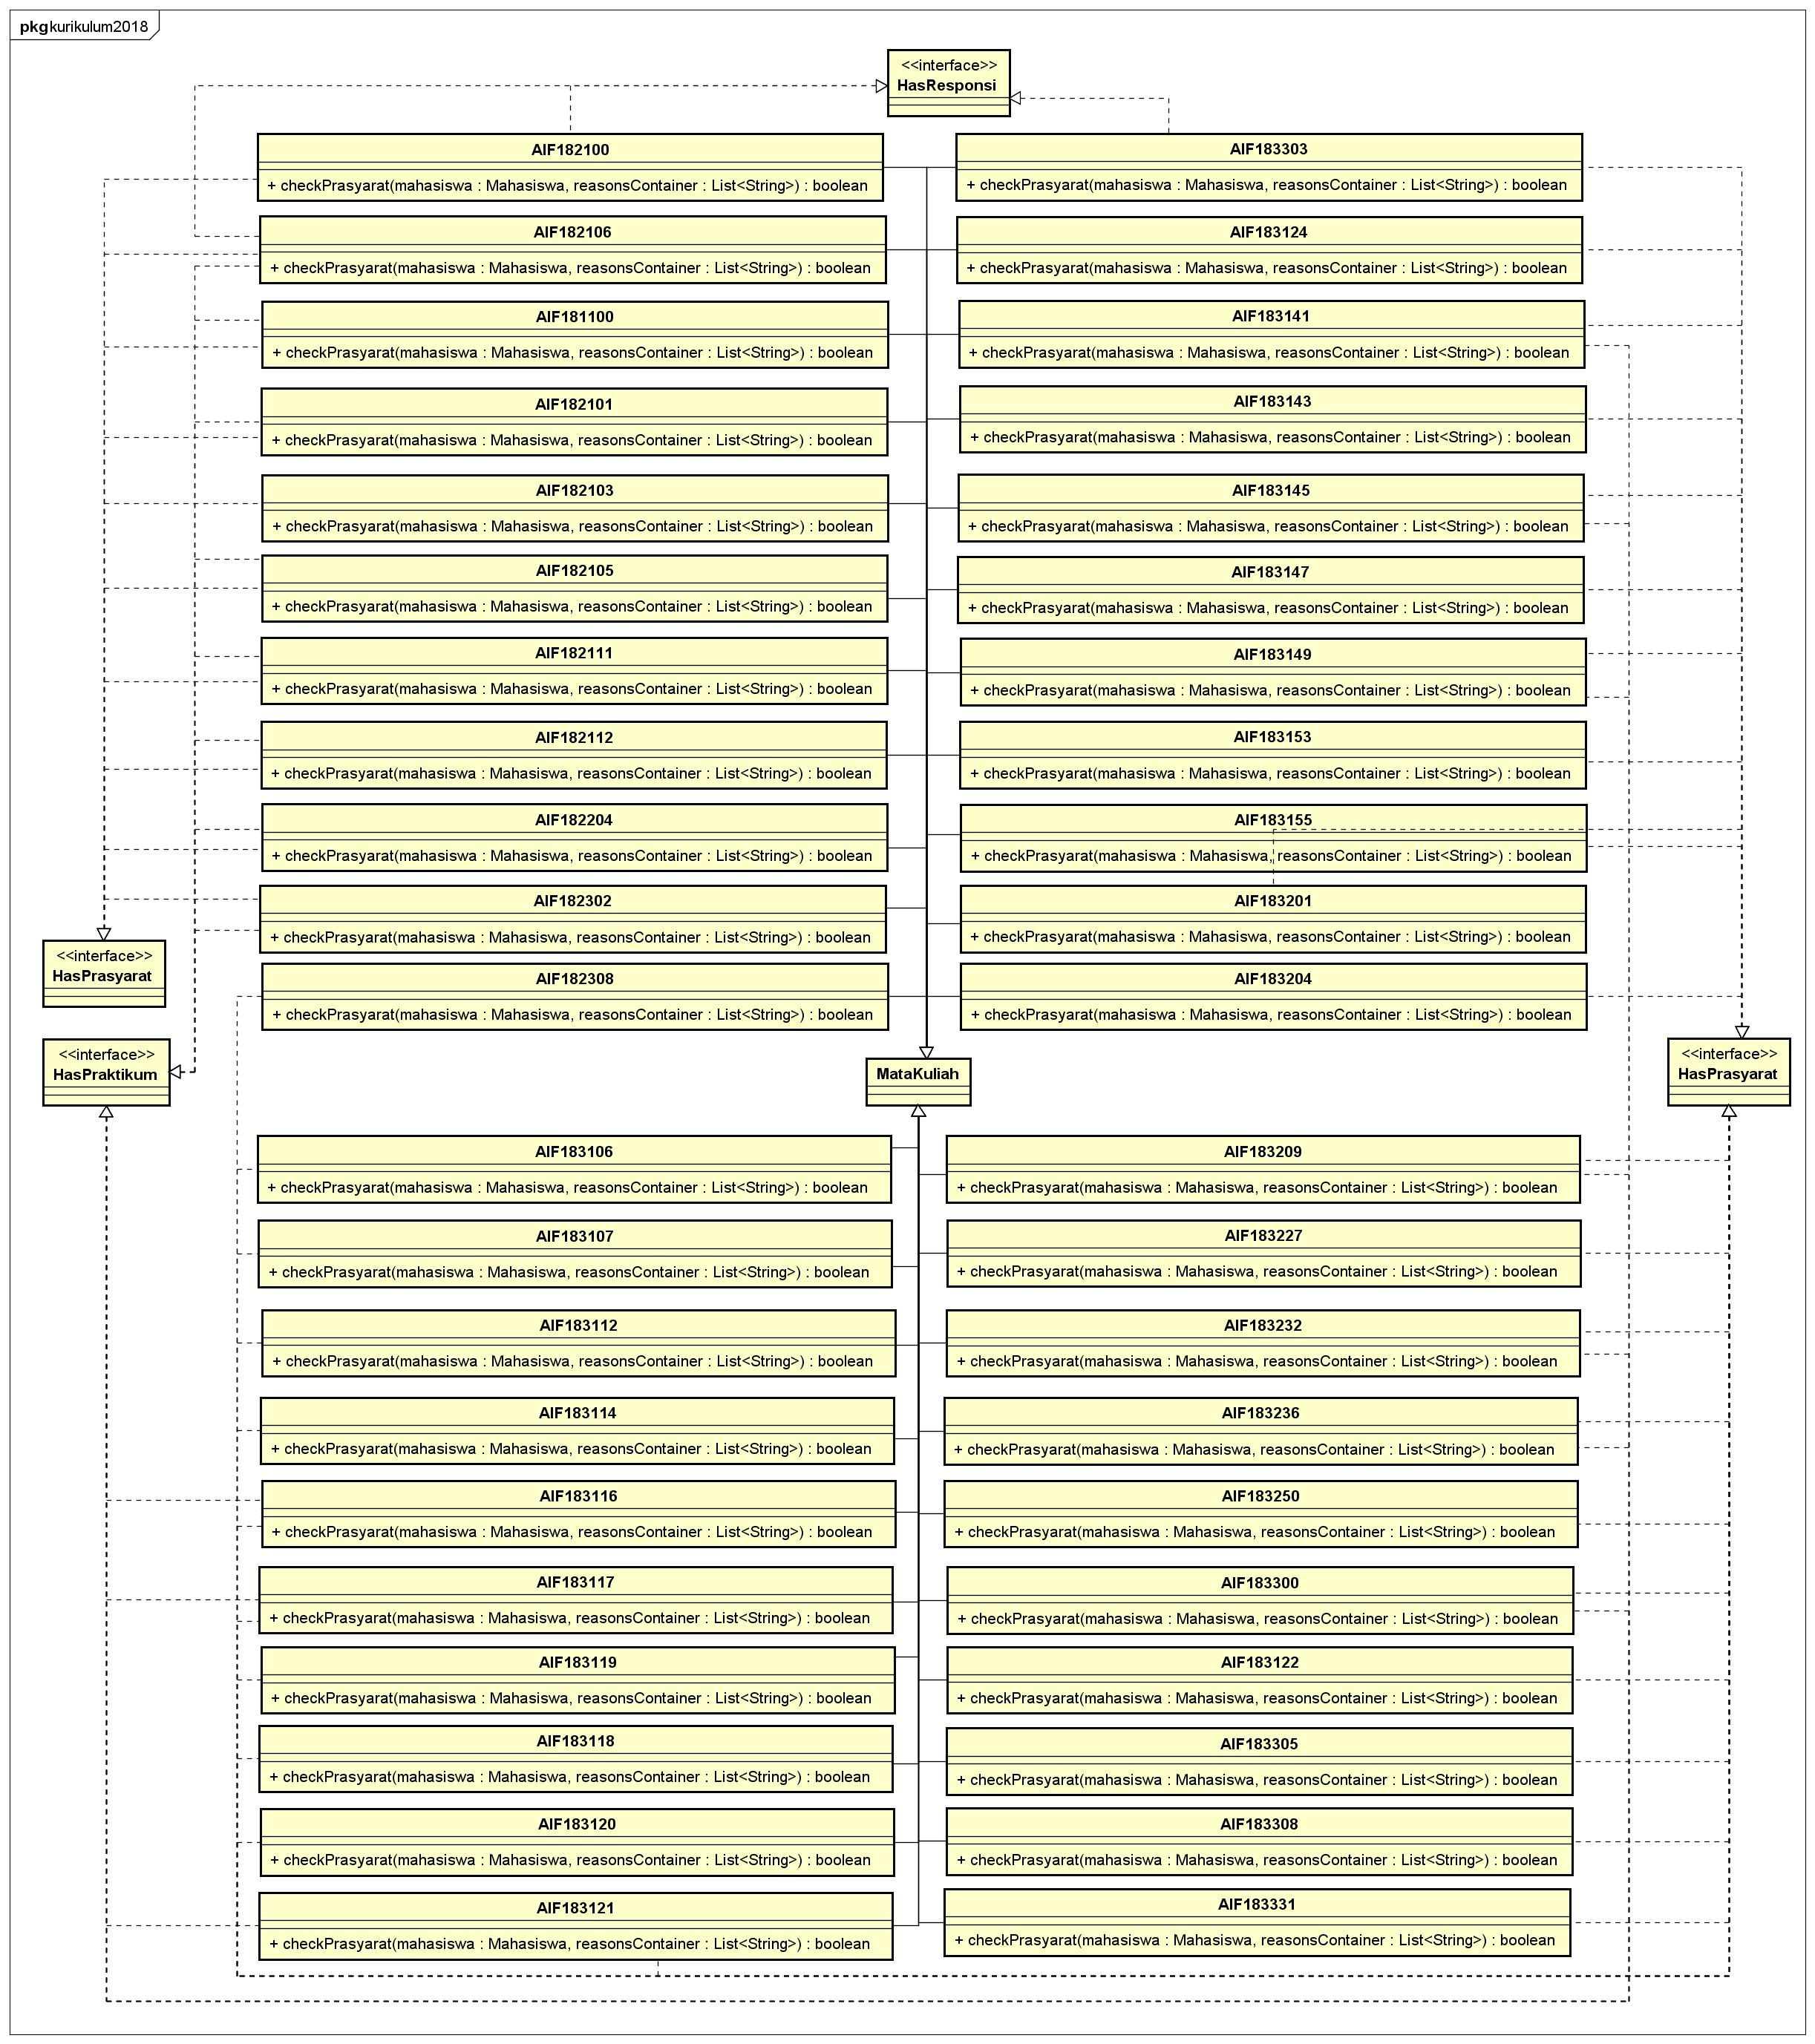
\includegraphics[scale=0.19]{Gambar/class-diagram-siamodels-mk-kurikulum-2018-4}
\caption{Diagram Kelas SIAModels \textit{Package} \texttt{kurikulum2018} (4/5)}
\label{fig:siamodels_class_2018_kurikulum_4}
\end{figure}

\begin{figure}[H]
\centering
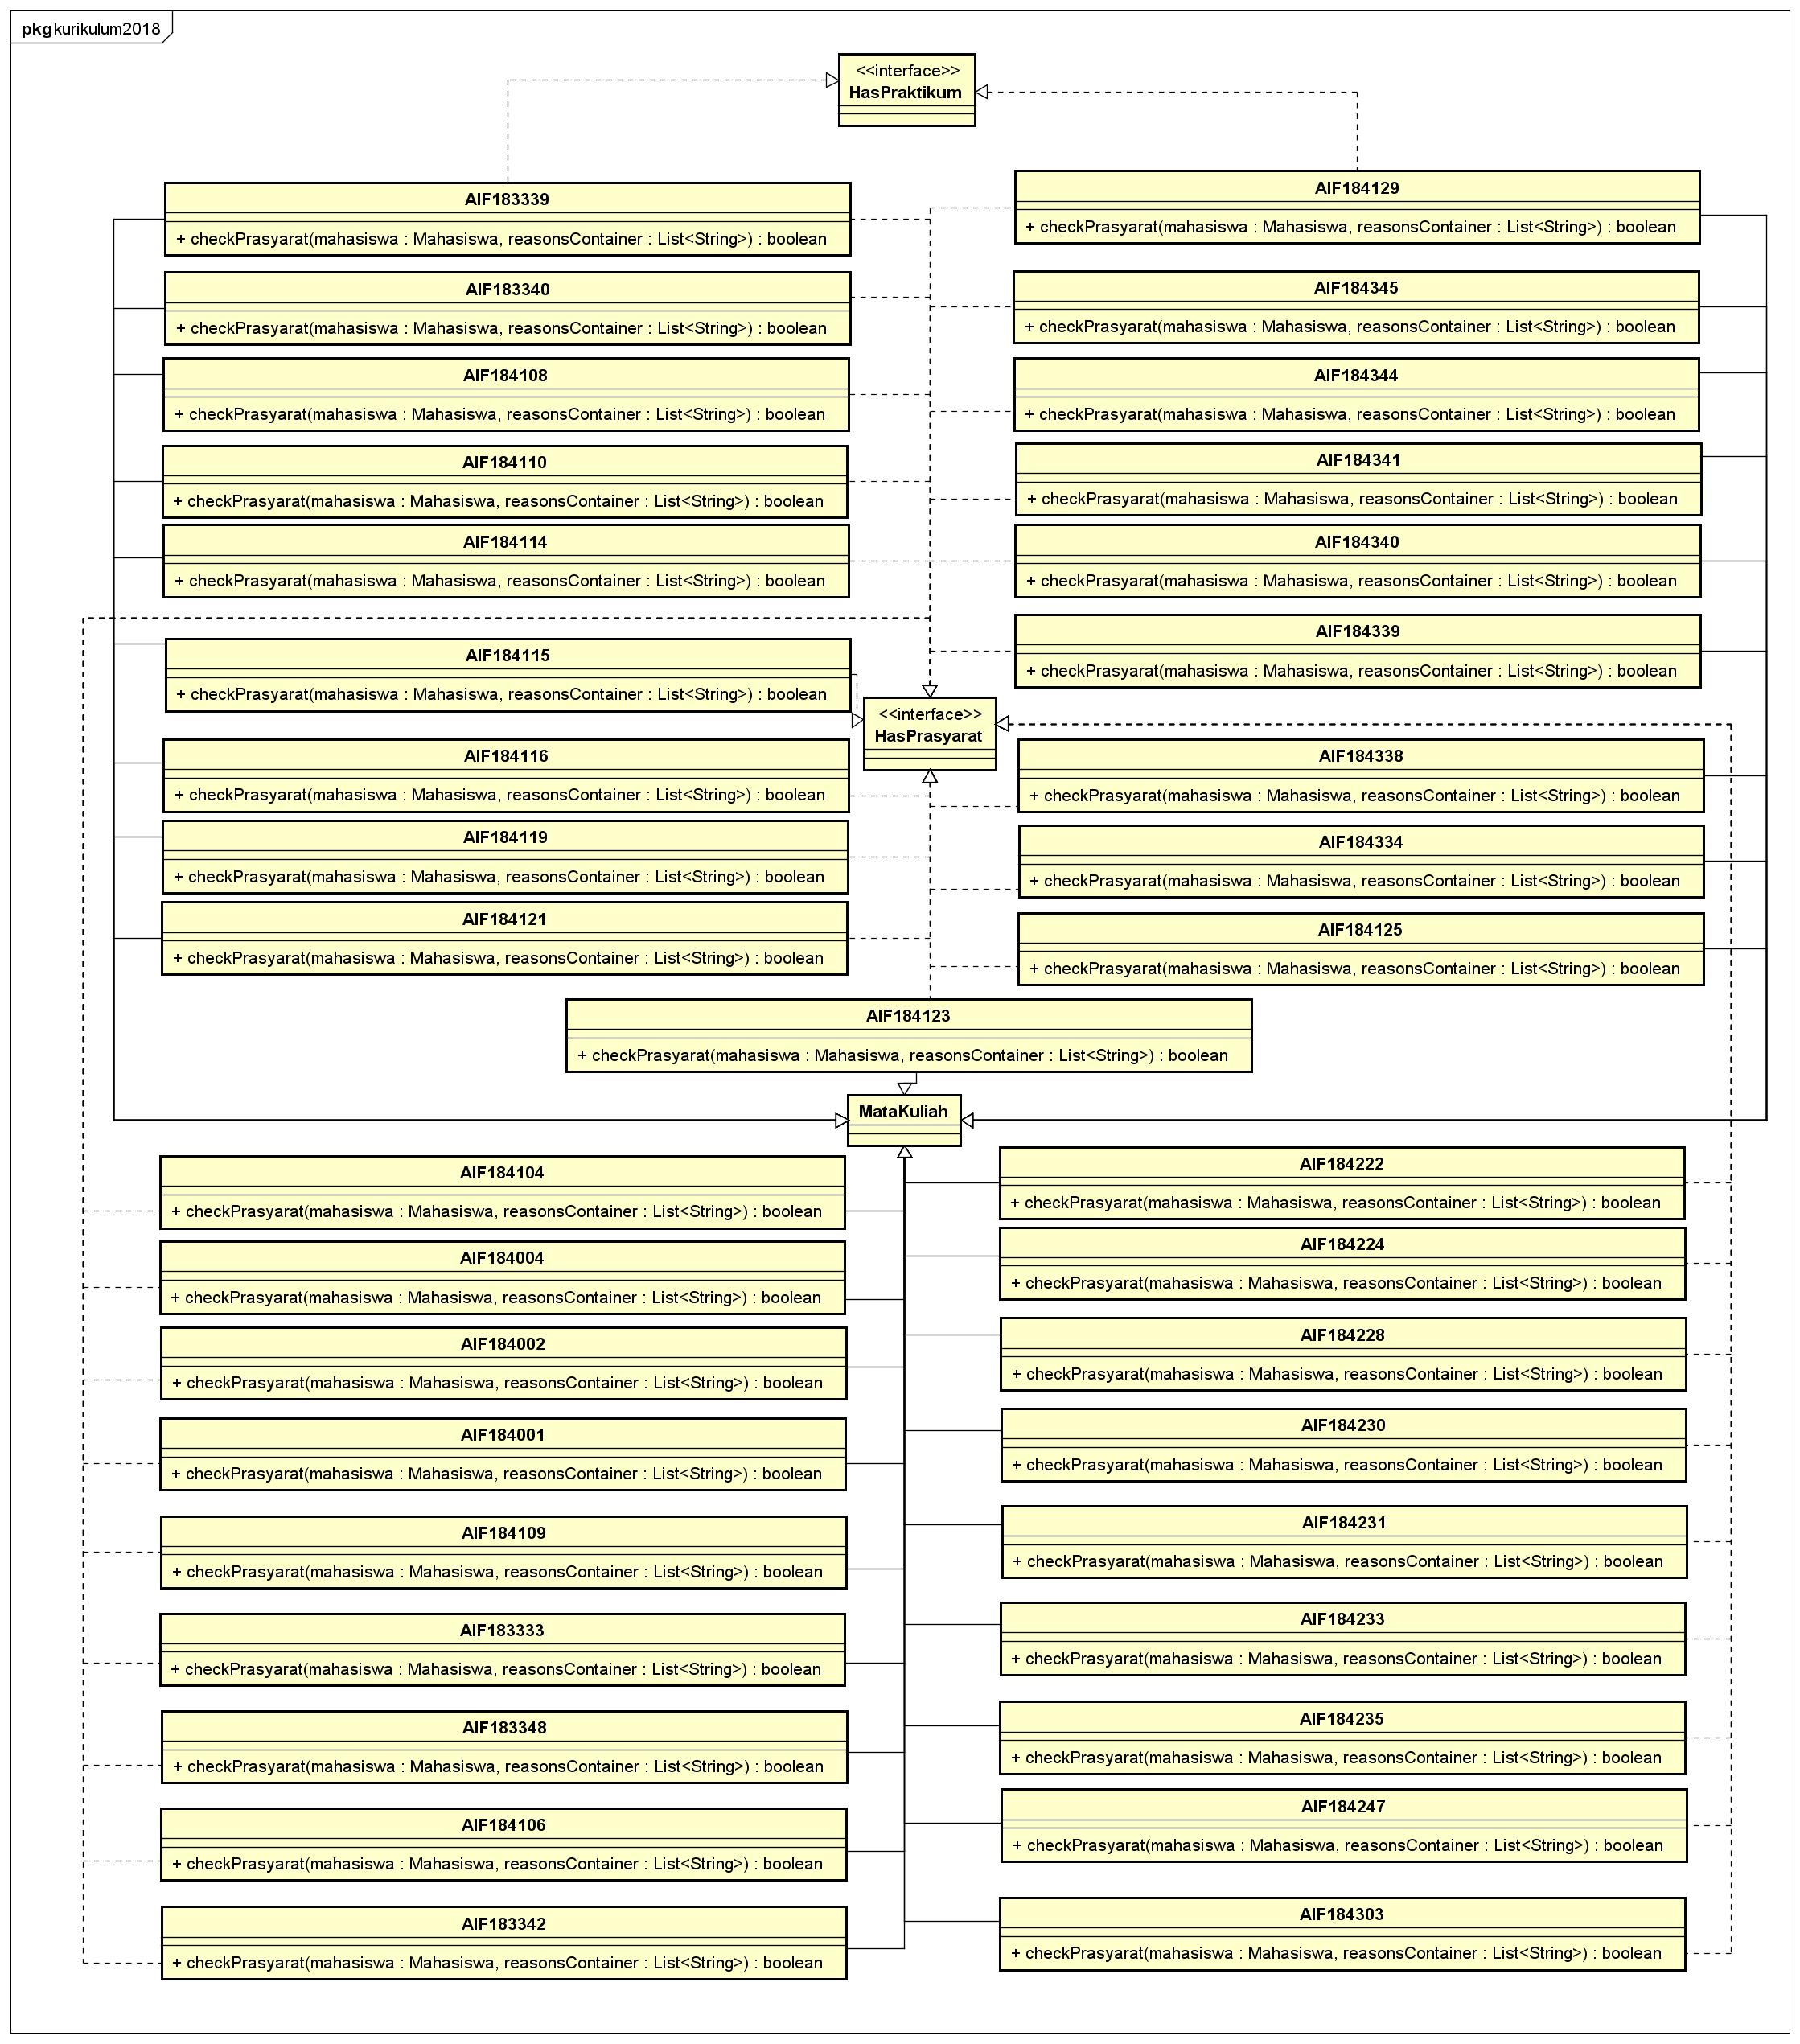
\includegraphics[scale=0.2]{Gambar/class-diagram-siamodels-mk-kurikulum-2018-5}
\caption{Diagram Kelas SIAModels \textit{Package} \texttt{kurikulum2018} (5/5)}
\label{fig:siamodels_class_2018_kurikulum_5}
\end{figure}

\begin{enumerate}
	\item \textit{Package} \texttt{id.ac.unpar.siamodels.matakuliah.kurikulum2018} \\
	\textit{Package} ini berisi kelas-kelas yang merepresentasikan mata kuliah pada kurikulum 2018 berserta aturan prasyaratnya. Kelas-kelas yang ada pada \textit{package} ini adalah sebagai berikut:
	\begin{table}[H]
\centering
\caption{Tabel rincian kelas mata kuliah kurikulum 2018}
\label{tab:kelasmatakuliah2018_rincian}
\begin{tabular}{|p{2cm}|p{3.5cm}|p{1.75cm}|p{2cm}|p{3.5cm}|p{1.75cm}|}
\hline
\textbf{Kelas} & \textbf{Nama} & \textbf{Prasyarat} & \textbf{Kelas} & \textbf{Nama} & \textbf{Prasyarat} \\ \hline
AIF131101 & Pemrograman Berorientasi Objek &  & AIF183145 & Sertifikasi Dasar-dasar Java & v \\ \hline
AIF131102 & Algoritma dan Struktur Data &  & AIF183147 & Teori Bilangan & v \\ \hline
AIF131105 & Pengantar Informatika &  & AIF183149 & Teori Bahasa \& Kompilasi & v \\ \hline
AIF131106 & Sistem Dijital &  & AIF183153 & Metode Numerik & v \\ \hline
AIF131181 & Dasar-dasar Pemrograman &  & AIF183155 & Pemrograman Lojik & v \\ \hline
AIF131182 & Pengantar Basis Data &  & AIF183201 & Sistem Operasi & v \\ \hline
AIF131183 & Pemrograman Prosedural &  & AIF183204 & Jaringan Komputer & v \\ \hline
AIF131191 & Pemrograman Berorientasi Objek &  & AIF183209 & Pemrograman pada Perangkat Bergerak & v \\ \hline
AIF131192 & Algoritma dan Struktur Data & & AIF183225 & Seritifikasi Administrasi Jaringan Komputer 1 & \\ \hline
AIF131195 & Pengantar Informatika &  & AIF183227 & Pengantar Telekomunikasi & v \\ \hline
AIF131198 & Logika Informatika & & AIF183229 & Topik Khusus Sistem Terdistribusi 1 & \\ \hline
AIF132202 & Desain dan Analisis Algoritma &  & AIF183232 & Pemrograman Berbasis Web Lanjut & v \\ \hline
AIF132205 & Arsitektur dan Organisasi Komputer &  & AIF183236 & Seritifikasi Administrasi Jaringan Komputer 2 & v \\ \hline
AIF132296 & Sistem Operasi &  & AIF183340 & Metodologi Pengembangan Sistem Informasi 2 & v \\ \hline
AIF132298 & Rekayasa Perangkat Lunak &  & AIF183342 & Kewirausahaan Berbasis Teknologi & v \\ \hline
AIF133305 & Jaringan Komputer & & AIF183346 & Topik Khusus Sistem Informasi 2 & \\ \hline
AIF133315 & Pemrograman Berbasis Web &  & AIF183348 & Sistem Kecerdasan Bisnis & v \\ \hline
AIF133317 & Desain Antarmuka Grafis & & AIF184000 & Etika Profesi & \\ \hline
AIF133318 & Pemrograman Aplikasi Bergerak &  & AIF184001 & Skripsi 1 & v \\ \hline
AIF133337 & Matematika Teknik &  & AIF184002 & Skripsi 2 & v \\ \hline
AIF133350 & Algoritma Genetika &  & AIF184004 & Tugas Akhir & v \\ \hline
AIF133352 & Jaringan Syaraf Tiruan & & AIF184005 & Komputer dan Masyarakat & \\ \hline
AIF133356 & Analisis Proses Bisnis & & AIF184006 & Kerja Praktek 4 & \\ \hline
AIF133380 & Teori Bahasa dan Otomata & & AIF184007 & Kerja Praktek 3 & \\ \hline
\end{tabular}
\end{table}

\begin{table}[H]
\centering
\label{tab:kelasmatakuliah2018_rincian_2}
\begin{tabular}{|p{2cm}|p{3.5cm}|p{1.75cm}|p{2cm}|p{3.5cm}|p{1.75cm}|}
\hline
\textbf{Kelas} & \textbf{Nama} & \textbf{Prasyarat} & \textbf{Kelas} & \textbf{Nama} & \textbf{Prasyarat} \\ \hline
AIF133381 & Analisis Sistem Informasi &  & AIF184104 & Bio-Inspired Computing & v \\ \hline
AIF133382 & Gudang Data dan Penambangan Data &  & AIF184106 & Pemrograman Permainan Komputer & v \\ \hline
AIF133383 & Praktika Grafika Komputer &  & AIF184108 & Kompresi Data & v \\ \hline
AIF133384 & Praktika Pemrograman Basis Data &  & AIF184109 & Pembelajaran Mesin & v \\ \hline
AIF133385 & Praktika Pemrograman Berbasis Web &  & AIF184110 & Pengolahan Citra & v \\ \hline
AIF133386 & Manajemen Proyek Teknologi Informasi &  & AIF184114 & Verifikasi Formal & v \\ \hline
AIF133388 & Praktika Pemrograman Aplikasi Bergerak &  & AIF184115 & Pencarian \& Temu Kembali Informasi & v \\ \hline
AIF133389 & Kriptografi &  & AIF184116 & Sistem Multi Agen & v \\ \hline
AIF134401 & Skripsi 1 &  & AIF184119 & Kecerdasan Buatan Untuk Permainan Komputer & v \\ \hline
AIF134402 & Skripsi 2 & & AIF184120 & Topik Khusus Informatika 4 & \\ \hline
AIF134443 & Matematika Kombinatorial &  & AIF184121 & Metode Optimisasi & v \\ \hline
AIF134448 & Pemrosesan Data Geografis &  & AIF184123 & Teknologi Mesin Pencari & v \\ \hline
AIF134451 & Audit Sistem Informasi &  & AIF184125 & Pengolahan Bahasa Alami & v \\ \hline
AIF134455 & Sistem Pendukung Keputusan & & AIF184127 & Topik Khusus Informatika 3 & \\ \hline
AIF134459 & Administrasi Basis Data &  & AIF184129 & Sertifikasi Administrasi Jaringan Komputer 3 & v \\ \hline
AIF134460 & Manajemen Pengetahuan &  & AIF184222 & Sertifikasi Administrasi Jaringan Komputer 4 & v \\ \hline
AIF134464 & Sistem Perusahaan Berskala Besar &  & AIF184224 & Sistem Terdistribusi & v \\ \hline
AIF134468 & Teknologi Multimedia &  & AIF184228 & Pemrograman Jaringan & v \\ \hline
AIF134471 & Metode Formal &  & AIF184230 & Keamanan Jaringan & v \\ \hline
AIF134480 & Pemrograman Sistem &  & AIF184231 & Jaringan Nirkabel & v \\ \hline
AIF134481 & Sistem Pakar & & AIF184232 & Topik Khusus Sistem Terdistribusi 4 & \\ \hline
AIF134483 & Teknik Kompilasi &  & AIF184233 & Teknologi Middleware & v \\ \hline
AIF134484 & Kewirausahaan &  & AIF184235 & Layanan Berbasis Web & v \\ \hline
AIF134487 & Perencanaan Sistem Informasi & & AIF184237 & Topik Khusus Sistem Terdistribusi 3 & \\ \hline
AIF134489 & Keamanan Informasi Dijital &  & AIF184247 & Jaringan Komputer Lanjut & v \\ \hline
\end{tabular}
\end{table}

\begin{table}[H]
\centering
\label{tab:kelasmatakuliah2018_rincian_3}
\begin{tabular}{|p{2cm}|p{3.5cm}|p{1.75cm}|p{2cm}|p{3.5cm}|p{1.75cm}|}
\hline
\textbf{Kelas} & \textbf{Nama} & \textbf{Prasyarat} & \textbf{Kelas} & \textbf{Nama} & \textbf{Prasyarat} \\ \hline
AIF181100 & Dasar Pemrograman & v & AIF184303 & Proyek Sistem Informasi 2 & v \\ \hline
AIF181101 & Pemodelan untuk Komputasi &  & AIF184334 & Sistem Informasi Skala Besar & v \\ \hline
AIF181103 & Matematika Dasar & & AIF184336 & Sistem e-Government & \\ \hline
AIF181104 & Logika Informatika &  & AIF184338 & Manajemen Proses Bisnis & v \\ \hline
AIF181105 & Pengantar Informatika &  & AIF184339 & Pengendalian \& Audit Teknologi Informasi & v \\ \hline
AIF181106 & Matriks dan Ruang Vektor &  & AIF184340 & Sistem Informasi Geografis & v \\ \hline
AIF181107 & Matematika Diskret &  & AIF184341 & Penambangan Data & v \\ \hline
AIF181202 & Arsitektur dan Organisasi Komputer & & AIF184342 & Topik Khusus Sistem Informasi 4 & \\ \hline
AIF182007 & Teknik Presentasi & & AIF184343 & Topik Khusus Sistem Informasi 3 & \\ \hline
AIF182100 & Analisis dan Desain Perangkat Lunak & v & AIF184344 & Analisis Big Data & v \\ \hline
AIF182101 & Algoritma dan Struktur Data & v & AIF184345 & Teknologi Big Data dan Cloud Computing & v \\ \hline
AIF182103 & Struktur Diskret & v & AMS131190 & Matematika Informatika &  \\ \hline
AIF182105 & Pemrograman Berorientasi Objek & v & AMS131191 & Kalkulus &  \\ \hline
AIF182106 & Desain dan Analisis Algoritma & v & AMS132290 & Aljabar Linear dan Matriks &  \\ \hline
AIF182109 & Statistika untuk Komputasi & & AMS133390 & Pemrograman Linear & \\ \hline
AIF182111 & Pemrograman Kompetitif 1 & v & APS133302 & Dunia Dijital dan Sains &  \\ \hline
AIF182112 & Pemrograman Kompetitif 2 & v & APS133309 & Dunia Dijital dan Sains &  \\ \hline
AIF182204 & Pemrograman Berbasis Web & v & EAA131101 & Akuntansi Keuangan Dasar 1 &  \\ \hline
AIF182210 & Pengantar Jaringan Komputer & & EAA131102 & Akuntansi Keuangan Dasar 2 & \\ \hline
AIF182302 & Manajemen Informasi dan Basisdata & v & ESA131101 & Akuntansi Keuangan Dasar &  \\ \hline
AIF182308 & Pengantar Sistem Informasi & v & ESM131101 & Pengantar Bisnis &  \\ \hline
AIF183002 & Penulisan Ilmiah & & ESM131105 & Manajemen & \\ \hline
AIF183010 & Kerja Praktek 2 & & MKU130001 & Pendidikan Pancasila & \\ \hline
AIF183013 & Kerja Praktek 1 & & MKU130002 & Pendidikan Kewarganegaraan & \\ \hline
AIF183015 & Pendidikan Pengabdian kepada Masyarakat & & MKU130003 & Agama Katolik & \\ \hline
AIF183106 & Proyek Informatika & v & MKU130004 & Fenomenologi Agama &  \\ \hline
\end{tabular}
\end{table}

\begin{table}[H]
\centering
\label{tab:kelasmatakuliah2018_rincian_4}
\begin{tabular}{|p{2cm}|p{3.5cm}|p{1.75cm}|p{2cm}|p{3.5cm}|p{1.75cm}|}
\hline
\textbf{Kelas} & \textbf{Nama} & \textbf{Prasyarat} & \textbf{Kelas} & \textbf{Nama} & \textbf{Prasyarat} \\ \hline
AIF183107 & Pengantar Sistem Cerdas & v & MKU130008 & Etika &  \\ \hline
AIF183111 & Interaksi Manusia Komputer & & MKU130009 & Bahasa Indonesia & \\ \hline
AIF183112 & Pengujian Perangkat Lunak & v & MKU130010 & Bahasa Inggris &  \\ \hline
AIF183114 & Algoritma Kriptografi & v & MKU130011 & Estetika &  \\ \hline
AIF183116 & Komputasi Paralel & v & MKU130012 & Logika &  \\ \hline
AIF183117 & Grafika Komputer & v & MKU180110 & Pendidikan Kewarganegaraan &  \\ \hline
AIF183118 & Komputasi Geometri & v & MKU180120 & Logika &  \\ \hline
AIF183119 & Keamanan Informasi & v & MKU180130 & Bahasa Indonesia &  \\ \hline
AIF183120 & Perancangan Permainan Komputer & v & MKU180240 & Etika &  \\ \hline
AIF183121 & Pemrograman Kompetitif 3 & v & MKU180250 & Pendidikan Pancasila &  \\ \hline
AIF183122 & Pemodelan \& Simulasi & v & MKU180360 & Estetika &  \\ \hline
AIF183123 & Topik Khusus Informatika 1 & & MKU180370 & Agama Katolik & \\ \hline
AIF183124 & Grafika Komputer Lanjut & v & MKU180380 & Fenomenologi Agama &  \\ \hline
AIF183128 & Topik Khusus Informatika 2 & & SAB133315 & Kewirausahaan & \\ \hline
AIF183141 & Pemrograman Fungsional & v & SIR131104 & Bahasa Jepang &  \\ \hline
AIF183143 & Pemodelan Formal & v & SPO131116 & Perekonomian Indonesia &  \\ \hline
\end{tabular}
\end{table}
	\begin{itemize}
		\item Untuk kelas mata kuliah yang memiliki prasayarat mempunyai \textit{method} \texttt{public boolean checkPrasyarat(Mahasiswa mahasiswa, List<String> reasonsContainer)}. \textit{Method} ini untuk memeriksa prasyarat-prasyarat dari kuliah, spesifik untuk mahasiswa yang dituju. Jika ada pesan-pesan khusus, akan ditambahkan pada parameter reasonsContainer.\\
			\textbf{Parameter:}
			\begin{itemize}
				\item \textbf{mahasiswa} prasyarat kuliah akan diperiksa spesifik pada mahasiswa ini.
				\item \textbf{reasonsContainer} jika pesan-pesan terkait prasyarat akan ditambahkan di sini.
			\end{itemize}
			\textbf{Kembalian:} \texttt{true} jika seluruh prasyarat dipenuhi, \texttt{false} jika tidak.
	\end{itemize}
	\item \textit{Package} \texttt{id.ac.unpar.siamodels.prodi.teknikinformatika}\\
	\textit{Package} ini memiliki kelas sebagai berikut:
	\begin{itemize}
		\item Kelulusan\\
		Kelas ini untuk memeriksa syarat kelulusan. Atribut yang berubah untuk kelas ini antara lain:
		\begin{itemize}
			\item \textbf{String[][] WAJIB:} kode mata kuliah wajib pada kurikulum 2018.
			\item \textbf{String[] AGAMA:} kode mata kuliah agama pada kurikulum 2018.
		\end{itemize}
		\textit{Method} yang berubah kelas ini sebagai berikut:
		\begin{itemize}
			\item \textbf{public boolean checkPrasyarat(Mahasiswa mahasiswa, List<String> reasonsContainer)}\\
			Pada \textit{method} ini ditambahkan kondisi apakah mahasiswa sudah lulus kuliah skripsi 1 dan 2 atau kuliah tugas akhir. jika belum lulus salah satu mata kuliah skripsi atau tugas akhir, maka mahasiswa tidak bisa lulus.
		\end{itemize}
	\end{itemize}
	
	\item \textit{Package} \texttt{id.ac.unpar.siamodels.matakuliah.interfaces}\\
	\textit{Package} ini memiliki beberapa \textit{interface} antara lain:
	\begin{itemize}
		\item HasPrasyarat\\
		Mendefinisikan kelas-kelas yang memiliki prasyarat, terkustomisasi untuk seorang mahasiswa. Atribut yang berubah untuk interfaces ini adalah sebagai berikut:
		\begin{itemize}
			\item \textbf{String[] DEFAULT\_HASPRASYARAT\_CLASSES:} Pada variabel ini terdapat perubahan nama kelas-kelas sesuai dengan mata kuliah yang memiliki prasyarat dalam kurikulum 2018.
		\end{itemize}
	\end{itemize}
	
	\item \textit{Package} \texttt{id.ac.unpar.siamodels}\\
	\textit{Package} ini memiliki kelas-kelas yang berubah akibat kurikulum 2018 adalah sebagai berikut:
	\begin{itemize}
			\item Mahasiswa\\
				Kelas ini merepresentasikan mahasiswa. \textit{Method-method} yang berubah untuk kelas ini adalah sebagai berikut:
				\begin{itemize}
					\item \textbf{public double calculateIPTempuh(boolean lulusSaja)}\\
						Pada \textit{method} ini yang berubah adalah ketika proses \textit{looping} untuk mencari nilai terbaik yang lulus pada setiap mata kuliah. Di dalam looping akan dilakukan pengecekan jika nilai akhir yang didapatkan adalah \textit{string} kosong, maka baris selanjutnya tidak akan dikerjakan lalu dilanjutkan dengan iterasi berikutnya.
					
					\item \textbf{public double calculateIPKumulatif()}\\
						Pada \textit{method} ini yang berubah adalah ketika proses \textit{looping} untuk mencari nilai untuk setiap mata kuliah. Di dalam looping akan dilakukan kondisi jika nilai akhir yang didapatkan adalah \textit{string} kosong, maka baris selanjutnya tidak akan dikerjakan kemudian dilanjutkan dengan iterasi berikutnya.
					
					\item \textbf{public int calculateSKSTempuh(boolean lulusSaja)}\\
						Pada \textit{method} ini yang berubah adalah ketika proses \textit{looping} untuk menambahkan jumlah sks setiap mata kuliah. Di dalam looping akan dilakukan kondisi jika nilai akhir yang didapatkan adalah \textit{string} kosong, maka baris selanjutnya tidak akan dikerjakan kemudian dilanjutkan dengan iterasi berikutnya.
					
					\item \textbf{public boolean hasLulusKuliah(String kodeMataKuliah)}\\
						Pada \textit{method} ini yang berubah adalah ketika proses \textit{looping} untuk mengetahui apakah mahasiswa sudah lulus mata kuliah tertentu terdapat sebuah kondisi jika nilai akhir tidak sama dengan \textit{string} kosong dan nilai akhir dibandingkan dengan nilai 'A' lebih besar sama dengan 0 dan nilai akhir dibandingkan dengan nilai 'D' lebih kecil sama dengan 0, maka akan mengembalikan nilai true.
		\end{itemize}
			
				\item Nilai\\
				Kelas ini merepresentasikan nilai yang ada pada riwayat nilai mahasiswa. Atribut yang berubah untuk kelas ini antara lain:
				\begin{itemize}
					\item \textbf{String nilaiAkhir:} tipe data nilaiAkhir berubah yang sebelumnya memiliki tipe data \textit{Character}.
				\end{itemize}
			\textit{Method-method} yang berubah untuk kelas ini adalah sebagai berikut:
				\begin{itemize}
					\item \textbf{public Nilai(TahunSemester tahunSemester, MataKuliah mataKuliah, Character kelas, Double nilaiART, Double nilaiUTS, Double nilaiUAS, String nilaiAkhir)}\\
						Pada \textit{Constructor} kelas \texttt{Nilai} terdapat perubahan pada parameter \textbf{nilaiAkhir} dari tipe data \textit{Character} menjadi tipe data \textit{String}.
						
					\item \textbf{public String getNilaikhir()}\\
						Pada \textit{method} ini tipe data berubaha menjadi tipe data \textit{String} yang sebelumnya tipe data \textit{Character}.
					
					\item \textbf{public Double getAngkaAkhir()}\\
						Pada \textit{method} ini nilai akhir akan diubah menjadi bobot nilai akhir. Perubahan yang terdapat \textit{method} ini adalah nilai akhir menjadi lebih bervariasi dan otomatis bobot nilai akhir akan mengikuti nilai akhir yang ada. Contohnya: terdapat nilai A- pada kurikulum 2018 yang memiliki bobot 3.67. 
				\end{itemize}
		\end{itemize}
\end{enumerate}

\section{Perancangan Protokol}
Pada bagian ini akan dijelaskan bagaimana memanfaatkan halaman-halaman di Student Portal untuk mendapatkan datanya. Halaman-halaman pada Student Portal yang dimanfaatkan IFStudentPortal.
\subsection{Halaman Home}
		\begin{figure}[H]
			\centering
			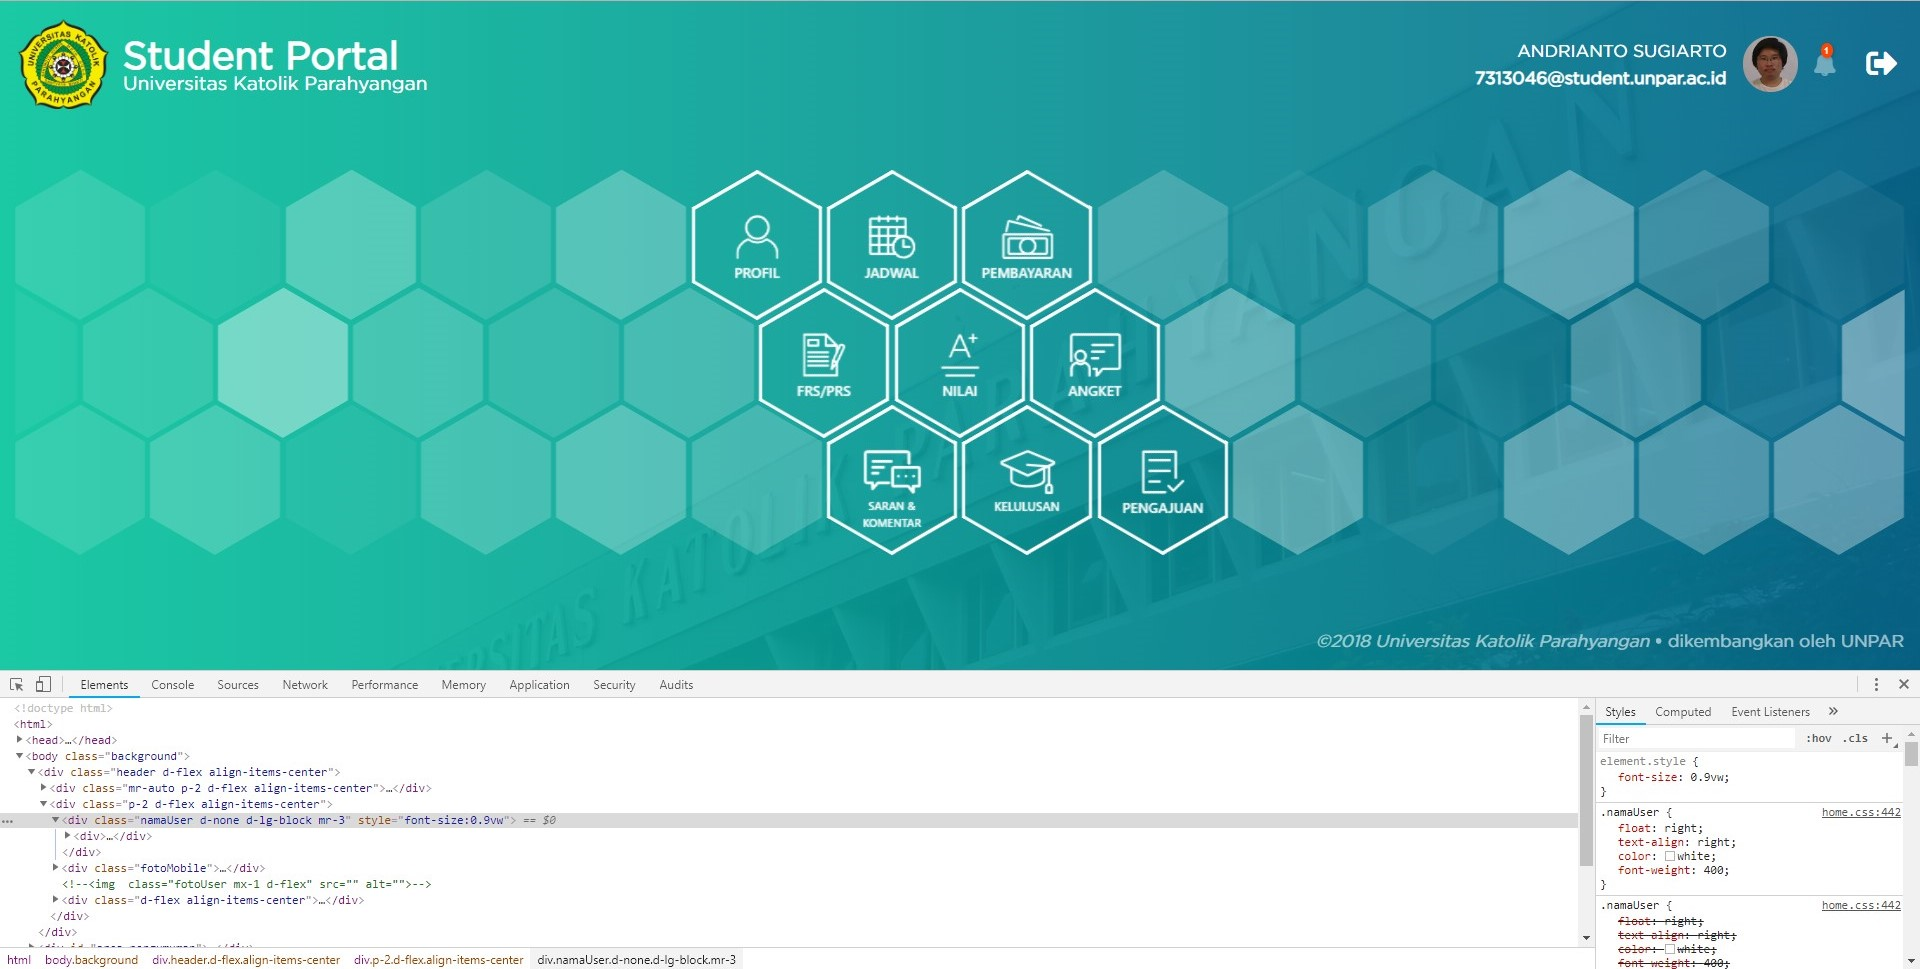
\includegraphics[scale=0.3]{Gambar/Home_nama_user}
			\caption{Elemen ``div.namaUser.d-none.d-lg-block.mr-3'' pada Halaman Home}
			\label{pic:home_nama_user}
		\end{figure}
		\begin{figure}[H]
			\centering
			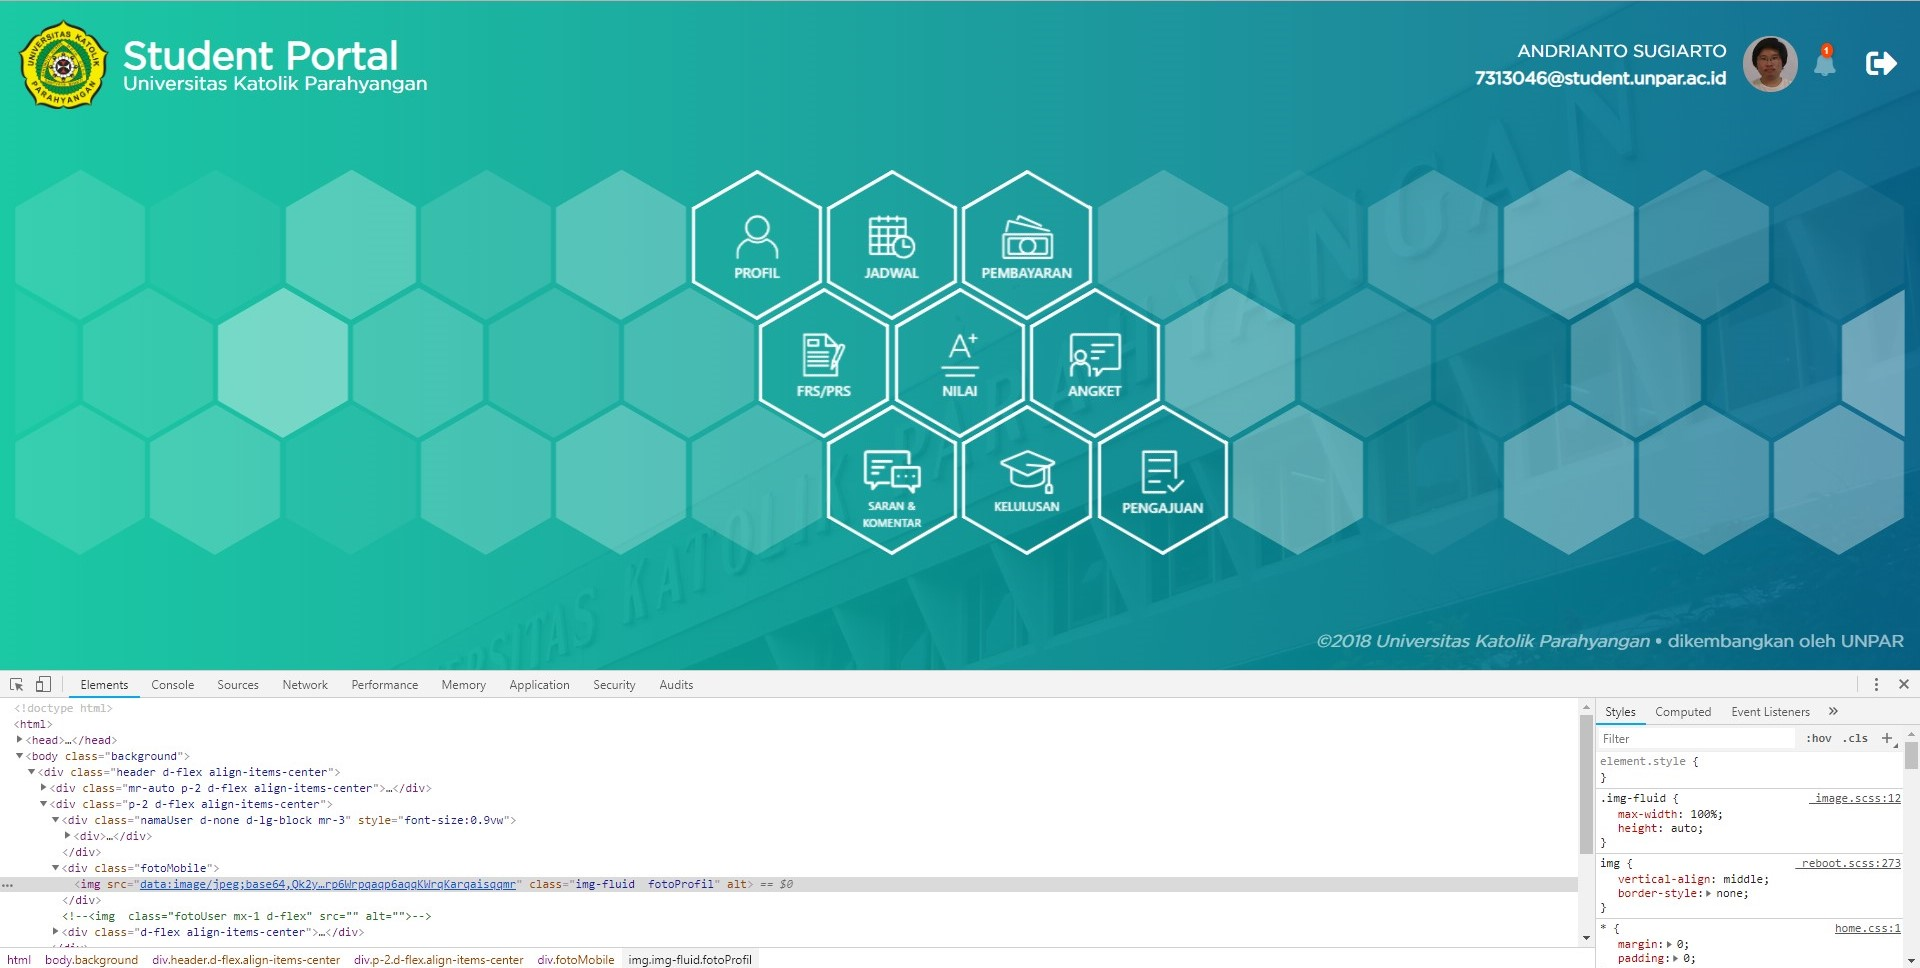
\includegraphics[scale=0.3]{Gambar/Home_foto_user}
			\caption{Elemen ``img.img-fluid.fotoProfil'' pada Halaman Home}
			\label{pic:home_foto_user}
		\end{figure}
Pada halaman ini terdapat data mahasiswa berupa nama dan foto mahasiswa yang didapatkan setelah login ke student portal. Data nama dan foto mahasiswa diproses menggunakan \textit{method} yang terdapat pada kelas \texttt{Scraper}, yaitu  \textit{method} \texttt{TahunSemester requestNamePhotoTahunSemester(String phpsessid, Mahasiswa mhs)}. Untuk memproses data nama dan foto mahasiswa dilakukan dengan cara:
\begin{enumerate}
	\item Melakukan koneksi ke \url{https://studentportal.unpar.ac.id/home}
	\item Setelah berhasil, mengambil data nama mahasiswa dengan melakukan kueri css menggunakan kueri ``div.namaUser.d-none.d-lg-block.mr-3'' (Gambar \ref{pic:home_nama_user})
	\item Setelah berhasil melakukan kueri css, akan mendapatkan nama dan email mahasiswa. Data yang dibutuhkan hanya nama mahasiswa, sehingga perlu memotong hasil kueri dari karakter pertama sampai indeks awal email mahasiswa. 
	\item Kemudian disimpan pada atribut kelas \texttt{Mahasiswa} dengan menggunakan \textit{method} \texttt{void setNama\\(String nama)}.
	\item Setelah berhasil menyimpan nama mahasiswa, kemudian melakukan kueri css untuk menyimpan foto mahasiswa menggunakan kueri ``img.img-fluid.fotoProfil'' (Gambar \ref{pic:home_foto_user})
	\item Setelah berhasil melakukan kueri css, akan mendapatkan foto mahasiswa dalam format \textit{Base64}. Disini perlu melakukan perubahan pada kelas \texttt{Mahasiswa}, yaitu:
	\begin{itemize}
		\item Atribut \texttt{URL photoUrl} menjadi \texttt{String photoPath}, karena data foto mahasiswa dalam format \textit{Base64}.
		\item \textit{Method} \texttt{URL getPhotoURL()} menjadi \\\texttt{String getPhotoPath()}, karena perubahan pada atribut dibutuhkan perubahan \textit{method getter}.
		\item \textit{Method} \texttt{void setPhotoURL(URL photoURL)} menjadi \texttt{void \\setPhotoPath(String photoPath)}, karena perubahan pada atribut dibutuhkan perubahan \textit{method setter}.
	\end{itemize}
	\item Kemudian disimpan pada atribut kelas \texttt{Mahasiswa} dengan menggunakan \textit{method} \texttt{void \\setPhotoPath(String photoPath)}
	\item Proses berikutnya akan dijelaskan pada sub sub-bab halaman FRS/PRS
\end{enumerate}

\subsection{Halaman FRS/PRS}
		\begin{figure}[H]
			\centering
			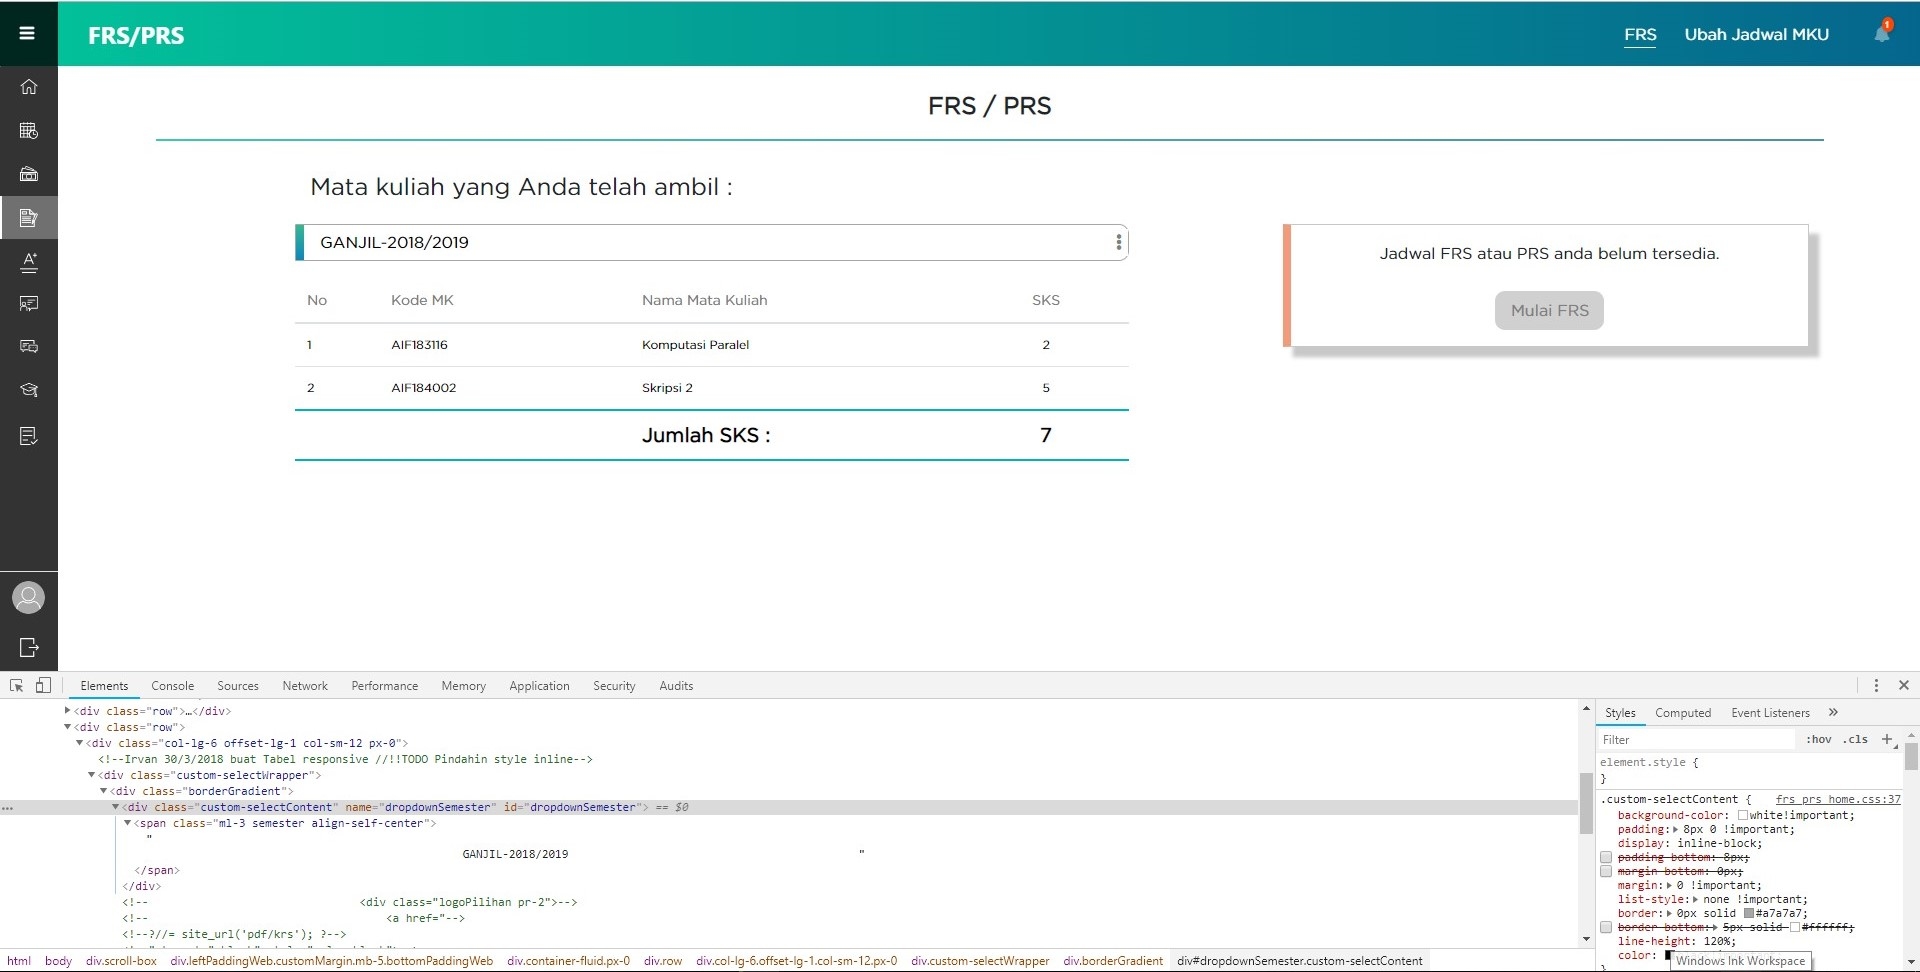
\includegraphics[scale=0.3]{Gambar/Home_semester_user}
			\caption{Elemen ``.custom-selectContent span'' pada Halaman FRS/PRS}
			\label{pic:home_semester_user}
		\end{figure}
Pada halaman ini terdapat data mahasiswa berupa tahun semester yang ditempuh oleh mahasiswa. Karena pada halaman home tidak bisa mendapatkan tahun semester yang ditempuh oleh mahasiswa, sehingga data tahun semester diambil dari halaman FRS/PRS. Data tahun semester diproses menggunakan \textit{method} yang terdapat pada kelas \texttt{Scraper}, yaitu  \textit{method} \texttt{TahunSemester requestNamePhotoTahunSemester(String phpsessid, Mahasiswa mhs)}. Untuk memproses data tahun semester dilakukan dengan cara:
\begin{enumerate}
	\item Melakukan koneksi ke \url{https://studentportal.unpar.ac.id/frs_prs}
	\item Setelah berhasil, mengambil data tahun semester mahasiswa dengan melakukan kueri css menggunakan kueri ``.custom-selectContent span'' (Gambar \ref{pic:home_semester_user})
	\item Setelah berhasil melakukan kueri css, akan didapatkan data tahun semester mahasiswa
	\item data tahun semester perlu diuraikan menjadi tahun dan semester yang disimpan pada \textit{array} tipe data \textit{String}, sehingga bisa disimpan pada atribut kelas \texttt{TahunSemester} dengan constructor \texttt{TahunSemester(int tahun, Semester semester)}
\end{enumerate}

\subsection{Halaman Jadwal}
		\begin{figure}[H]
			\centering
			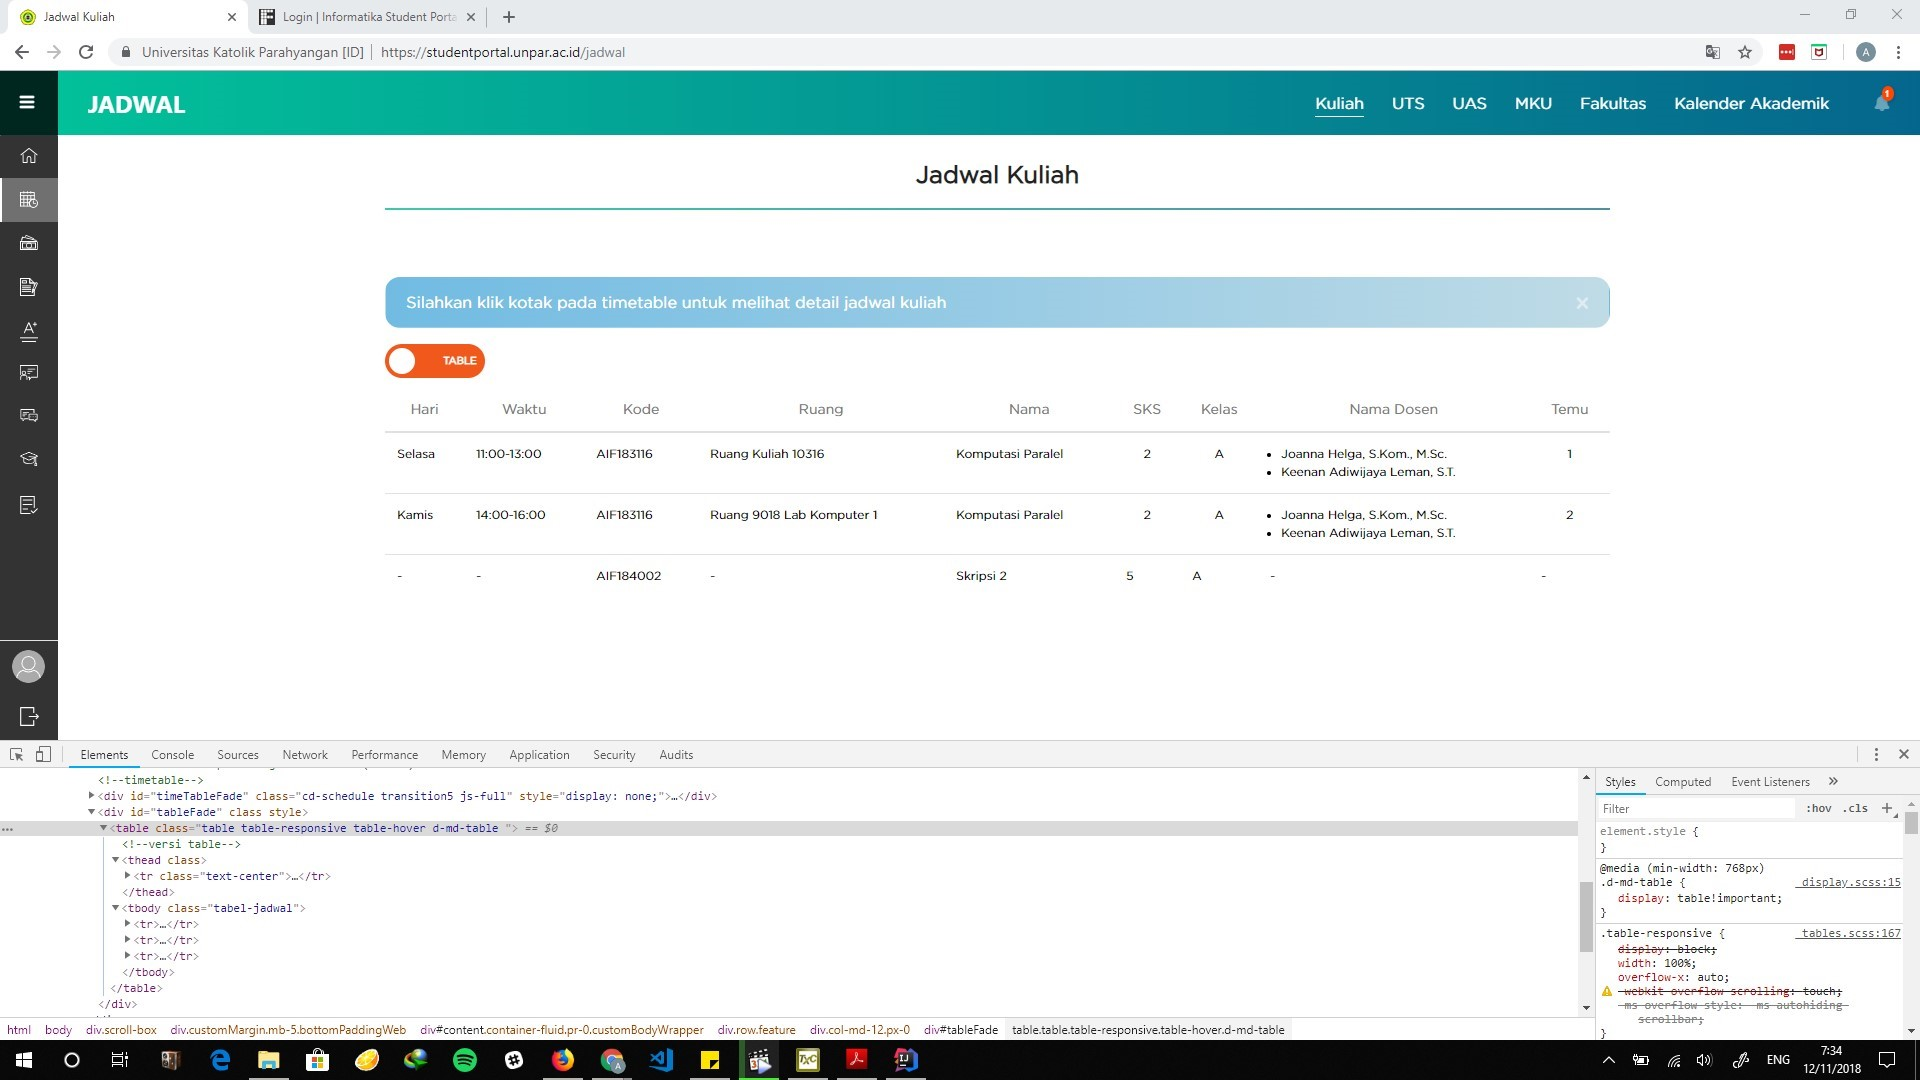
\includegraphics[scale=0.3]{Gambar/Jadwal_user}
			\caption{Elemen ``table.table.table-responsive.table-hover.d-md-table'' pada Halaman Jadwal}
			\label{pic:jadwal_user}
		\end{figure}
Pada halaman ini terdapat data jadwal kuliah dari mahasiswa. Data jadwal kuliah yang dibutuhkan untuk fitur jadwal kuliah pada IFStudentPortal diambil dari tampilan jadwal dalam bentuk tabel. Data jadwal kuliah diproses menggunakan \textit{method} yang terdapat pada kelas \texttt{Scraper}, yaitu  \textit{method} \texttt{List<JadwalKuliah> requestJadwal(String phpsessid)}. Untuk memproses data jadwal kuliah dilakukan dengan cara:
\begin{enumerate}
	\item Melakukan koneksi ke \url{https://studentportal.unpar.ac.id/jadwal}
	\item Setelah berhasil, mengambil data jadwal kuliah dengan melakukan kueri css menggunakan kueri ``table.table.table-responsive.table-hover.d-md-table'' (Gambar \ref{pic:jadwal_user}).
	\item Setelah berhasil melakukan kueri css, jika terdapat jadwal kuliah, maka jadwal kuliah diolah dan kemudian disimpan dalam sebuah daftar jadwal kuliah yang kemudian akan dikembalikan dalam bentuk daftar jadwal kuliah. 
\end{enumerate}

\subsection{Halaman Nilai}
		\begin{figure}[H]
			\centering
			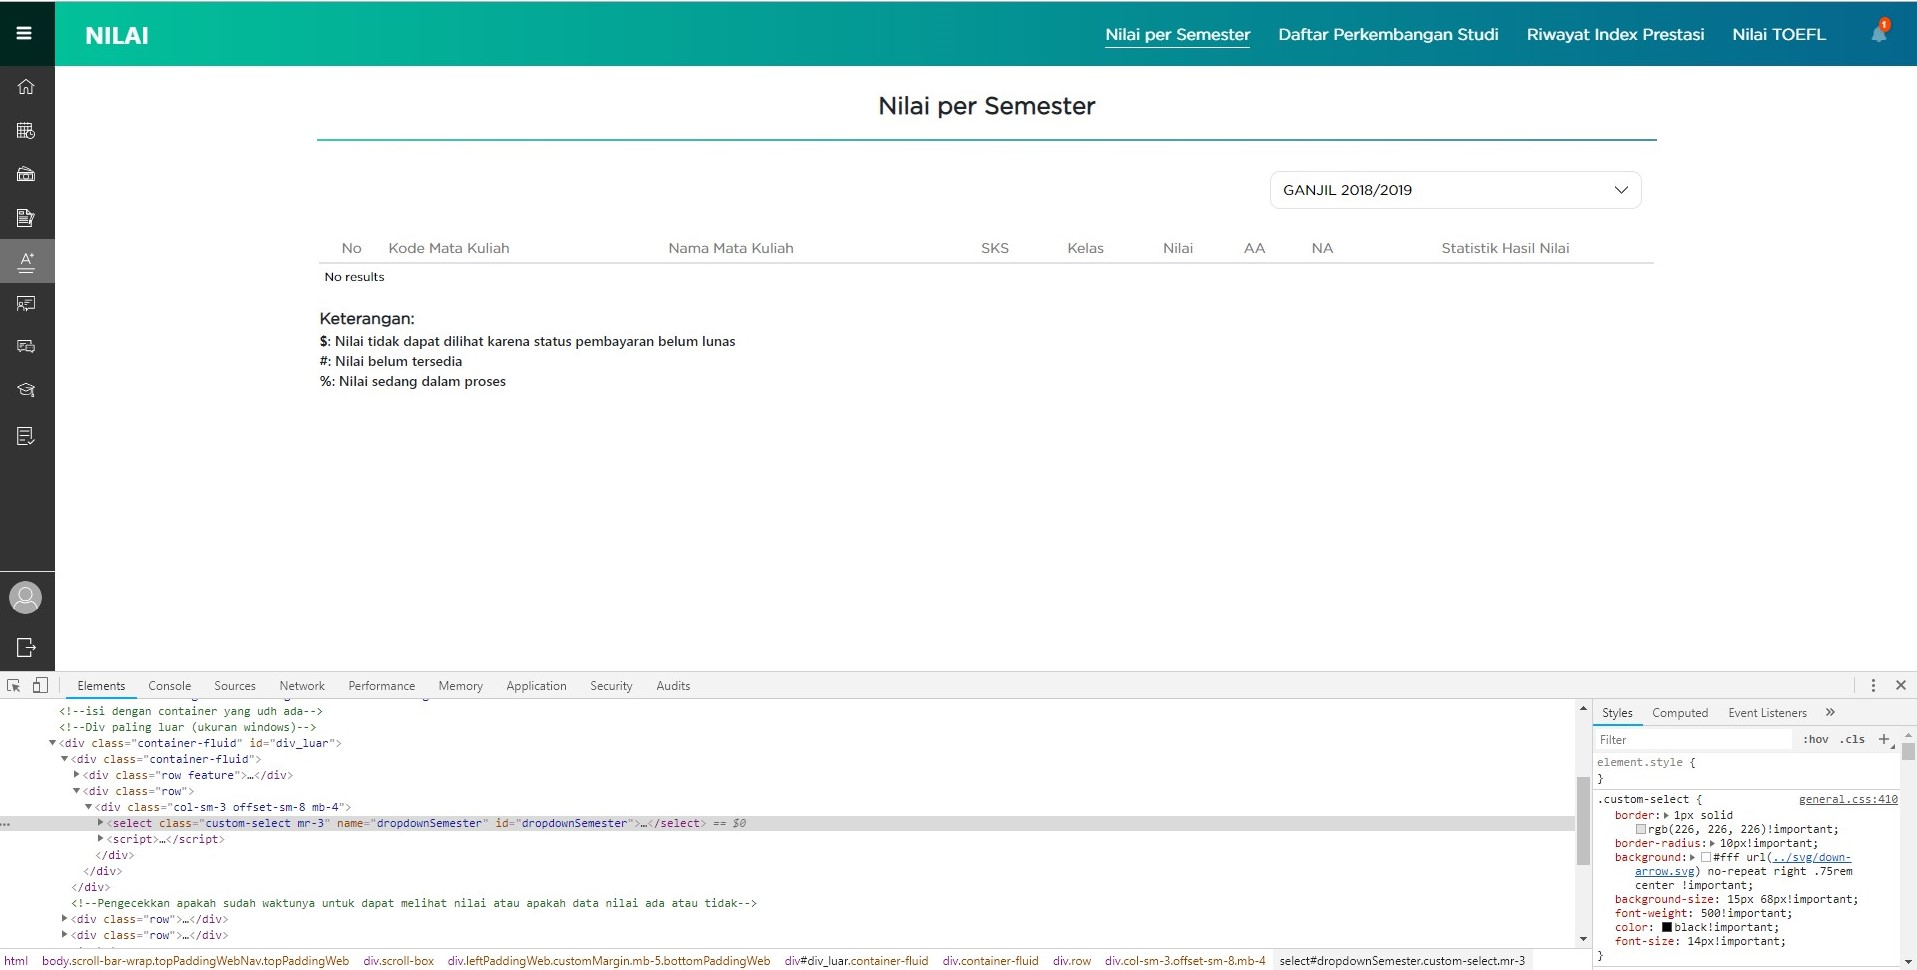
\includegraphics[scale=0.3]{Gambar/Nilai_combobox_user}
			\caption{\textit{Combo Box} ``select\#dropdownSemester.custom-select.mr-3'' pada Halaman Nilai}
			\label{pic:nilai_combobox_user}
		\end{figure}
Pada halaman ini terdapat data nilai mahasiswa terkini. Nilai yang diambil adalah nilai per semester yang sudah memuat kode mata kuliah yang berlaku di kurikulum 2018. Data nilai akan diproses menggunakan \textit{method} pada kelas \texttt{Scraper}, yaitu \textit{method} \texttt{void requestNilai(String phpsessid, Mahasiswa logged\_mhs)}. Untuk memproses daata nilai dilakukan dengan cara:
\begin{enumerate}
	\item Melakukan koneksi ke \url{https://studentportal.unpar.ac.id/nilai}
	\item Setelah berhasil, mengambil data nilai berdasarkan tahun dan semester dengan melakukan kueri css menggunakan kueri ``select\#dropdownSemester.custom-select.mr-3'' (Gambar \ref{pic:nilai_combobox_user})
	\item Setelah berhasil melakukan kueri css, kemudian disimpan pada atribut lokal \texttt{ArrayList<String> listSemester} dari atribut \textit{value} ``\textit{option}''
	\item Setelah berhasil menyimpan \textit{value ``option''} dari \textit{Combo Box}. Kemudian diperlukan melakukan koneksi berkali-kali sebanyak semester yang telah ditempuh mahasiswa, sehingga dibutuhkan waktu yang tidak sebentar. Karena pada halaman nilai tidak dapat menampilkan seluruh semester seperti Student Portal yang lama, sehingga untuk mengatasi masalah ini dibuat menjadi paralel. Untuk itu dibuat kelas yang mengimplementasikan kelas \textit{interface} \texttt{Runnable}, yaitu:
	\begin{itemize}
		\item \texttt{MultipleRequest}
		\begin{figure}[H]
			\centering
			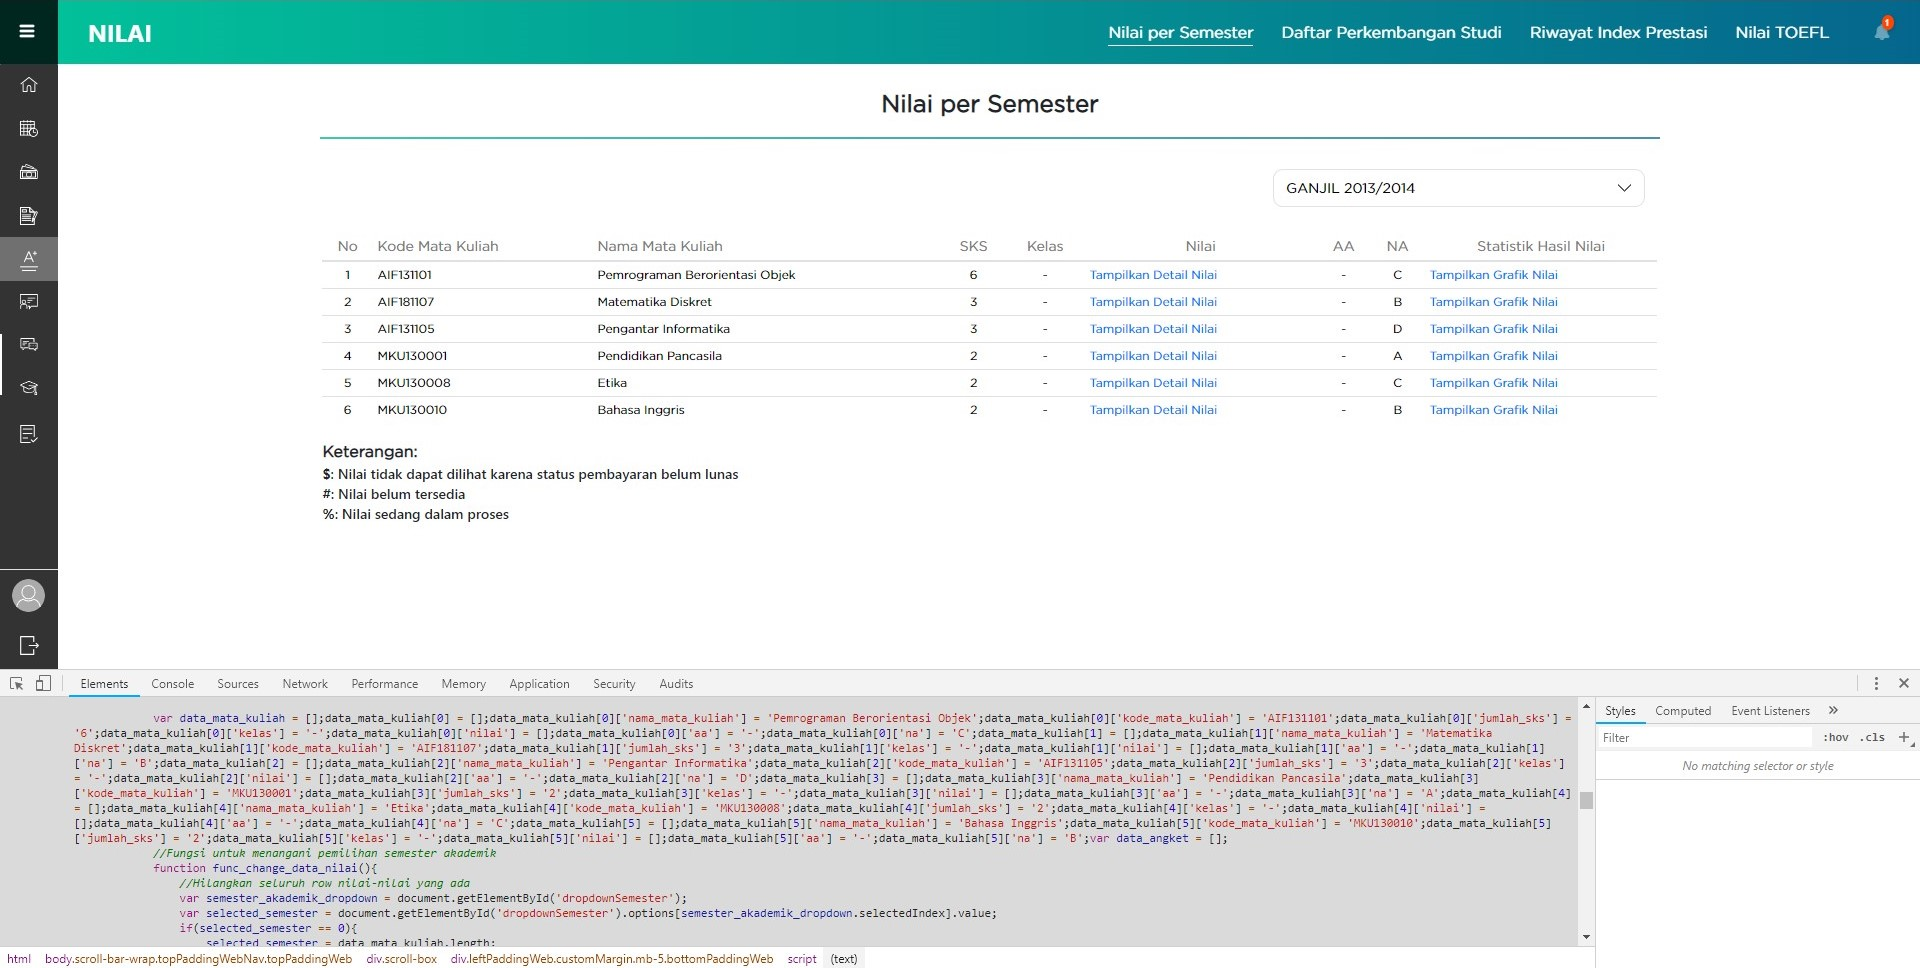
\includegraphics[scale=0.3]{Gambar/Nilai_per_semester_salah_satu}
			\caption{Script Data Nilai Mahasiswa Pada Halaman Nilai}
			\label{pic:nilai_per_semester_script}
		\end{figure}
		Pada kelas ini juga mengatasi masalah pengambilan data nilai dimana nilai di isi ke dalam tabel menggunakan \textit{javascript}. Atribut pada kelas ini merupakan atribut yang diperlukan untuk mendapatkan nilai mahasiswa, yaitu:
		\begin{itemize}
			\item Atribut \texttt{int l} merupakan atribut untuk menyimpan satu angka urutan dari atribut \texttt{listSemester}.
			\item Atribut \texttt{ArrayList<String> listSemester} merupakan daftar semester yang telah ditempuh mahasiswa.
			\item Atribut \texttt{String NILAI\_URL} merupakan alamat untuk mendapatkan nilai mahasiswa.
			\item Atribut \texttt{String phpsessid} untuk menyimpan \textit{cookies} dari \textit{login} ke Student Portal.
			\item Atribut \texttt{Mahasiswa logged\_mhs} untuk menyimpan data mahasiswa.
			\item Atribut \texttt{ScriptEngineManager factory} untuk menjalankan \textit{javascript}.
			\item Atribut \texttt{ScriptEngine engine} untuk menjalankan \textit{javascript}.
		\end{itemize}
		\textit{Method} yang dimiliki kelas ini adalah \texttt{void run}. \textit{Method} ini merupakan \textit{method} turunan dari kelas \texttt{interface Runnable}. Untuk mendapatkan data nilai dilakukan dengan cara:
		\begin{enumerate}
			\item Mendapatkan tahun dan semester yang ditempuh mahasiswa dari atribut \texttt{Arraylist\\<String> listSemester} diambil dari value atribut \texttt{int l}. Kemudian String dibagi menjadi tahun dan semester yang dibutuhkan.
			\item Setelah mendapatkan tahun dan semester. Kemudian melakukan koneksi ke alamat nilai berdasarkan tahun dan semester (\url{https://studentportal.unpar.ac.id/nilai/2013/1}).
			\item Setelah berhasil, kemudian melakukan kueri css berdasarkan script yang mengandung nilai mahasiswa (Gambar \ref{pic:nilai_per_semester_script}). 
			\item Selanjutnya adalah mendapatkan script yang mengandung script ``var data\_mata\_kuliah = [];'' sampai indeks dari ``var data\_angket = [];''.
			\item Setelah mendapatkan script yang dibutuhkan, selanjutnya menjalankan script menggunakan \textit{method} milik kelas \texttt{ScriptEngine} yaitu \texttt{Object eval(String script)}.
			\item Setelah berhasil, data yang didapatkan bertipe \texttt{ScriptObjectMirror} yang membungkus hasil eksekusi. Data nilai didapatkan dengan menggunakan \textit{method} \texttt{Object get(Object key)}.
			\item Setelah berhasil, kemudian memasukan data nilai ke daftar riwayat nilai mahasiswa pada atribut kelas \texttt{Mahasiswa} yaitu \texttt{List<Nilai> riwayatNilai} menggunakan method \texttt{List<Nilai> getRiwayatNilai()}. Proses ini dilakukan berulang kali sebanyak jumlah mata kuliah per semesternya.
		\end{enumerate}
	\end{itemize}
	\item Setelah berhasil mendapatkan seluruh nilai, kemudian data diurutkan berdasarkan tahun semester mata kuliah tersebut ditempuh.
\end{enumerate}

\subsection{Halaman Nilai TOEFL}
		\begin{figure}[H]
			\centering
			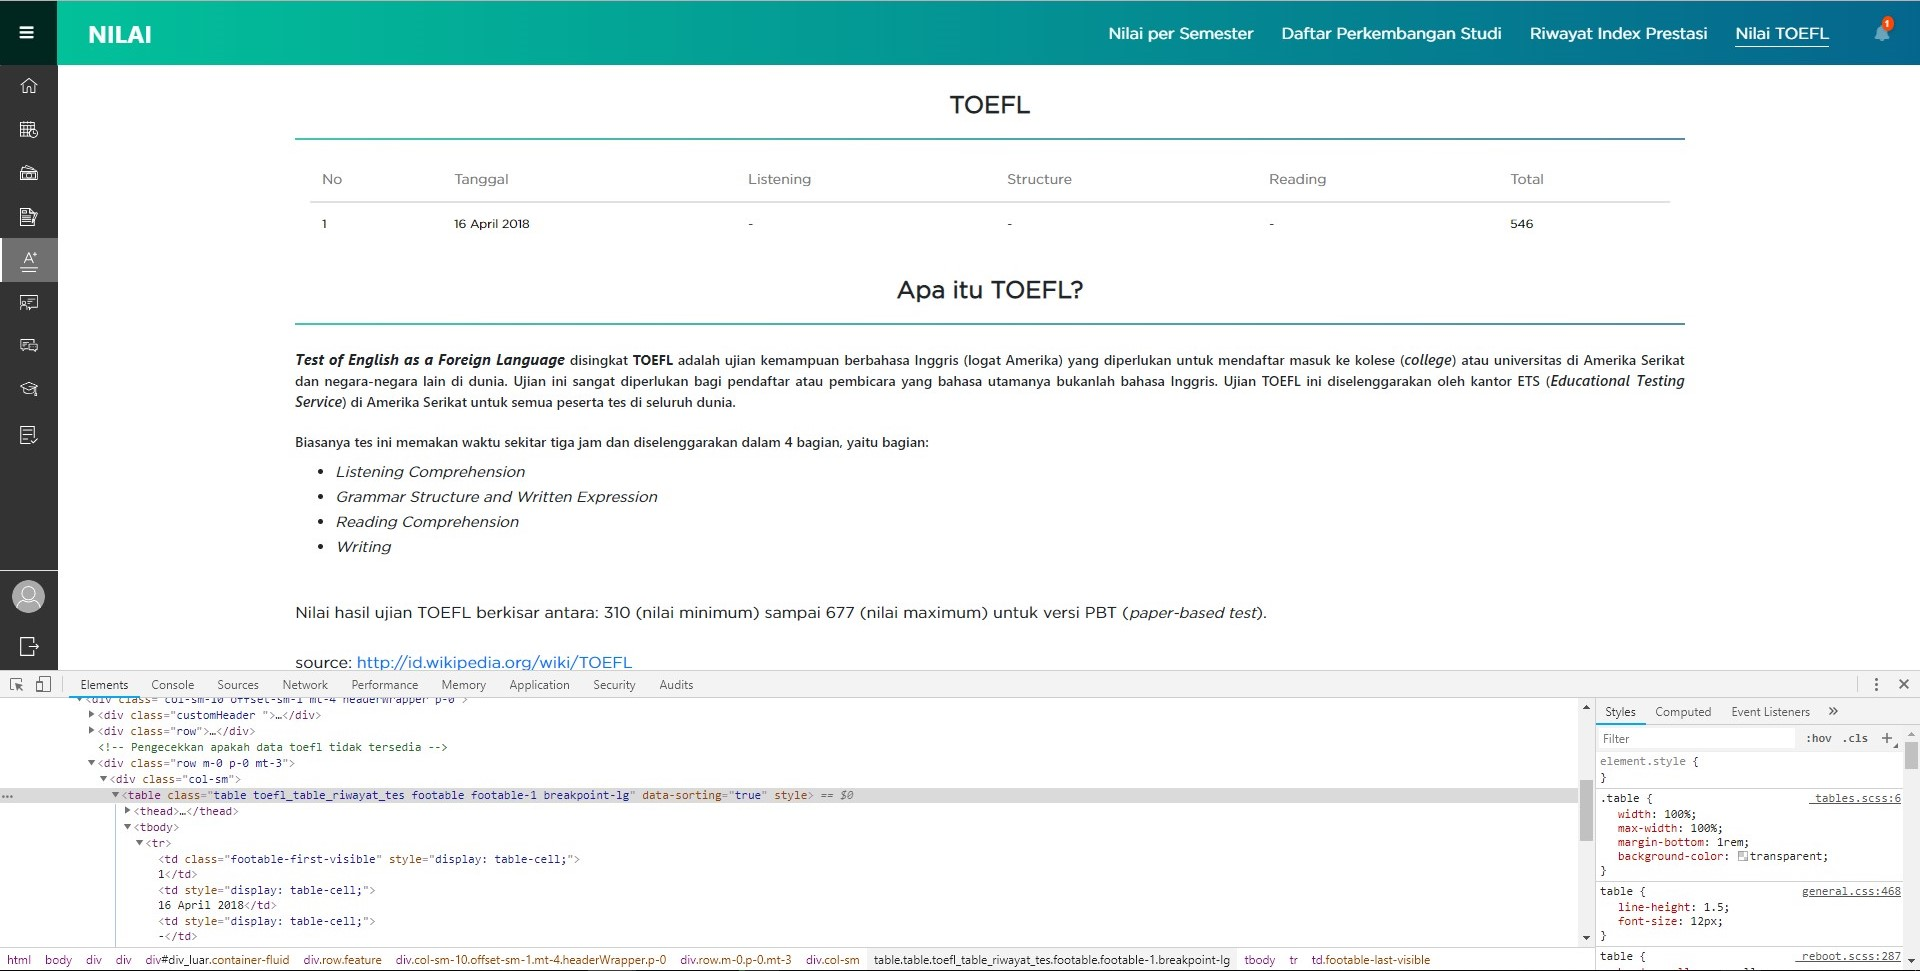
\includegraphics[scale=0.3]{Gambar/Nilai_toefl_css}
			\caption{Elemen ``table tbody tr'' dengan nilai TOEFL Mahasiswa}
			\label{pic:nilai_toefl_css}
		\end{figure}
Pada halaman ini terdapat data nilai TOEFL yang telah ditempuh oleh mahasiswa. Data nilai TOEFL akan diproses menggunakan \textit{method} pada kelas \texttt{Scraper}, yaitu \textit{method} \texttt{void requestNilaiTOEFL\\(String phpsessid, Mahasiswa mahasiswa)}. Untuk memproses data nilai TOEFL dilakukan dengan cara:
\begin{enumerate}
	\item Melakukan koneksi ke \url{https://studentportal.unpar.ac.id/nilai/toefl}
	\item Setelah berhasil, mengambil data nilai TOEFL dengan melakukan kueri css menggunakan kueri ``table'', ``tbody'', dan ``tr'' (Gambar \ref{pic:nilai_toefl_css})
	\item Setelah berhasil melakukan kueri css, akan mendapatkan data nilai TOEFL yang perlu diolah kemudian disimpan pada atribut kelas \textit{Mahasiswa} dengan menggunakan \textit{method} \texttt{void setNilaiTOEFL(SortedMap<LocalDate, Integer> nilaiTOEFL)}
\end{enumerate}

\section{Perancangan Antarmuka}
Pada subbab Perancangan Antarmuka tidak dilakukan perubahan terhadap tampilan antarmuka IFStudentPortal. Proses pengerjaan penelitian ini lebih fokus dalam penyesuaian IFStudentPortal dan SIAModels ke kurikulum 2018.